% Soubory musí být v kódování, které je nastaveno v příkazu \usepackage[...]{inputenc}

\documentclass[%
%  draft,    				  % Testovací překlad
  12pt,       				% Velikost základního písma je 12 bodů
  a4paper,    				% Formát papíru je A4
%  oneside,      			% Jednostranný tisk (výchozí)
%% Z následujicich voleb lze použít maximálně jednu:
%	dvipdfm  						% výstup bude zpracován programem 'dvipdfm' do PDF
%	dvips	  						% výstup bude zpracován programem 'dvips' do PS
%	pdftex							% překlad bude proveden programem 'pdftex' do PDF (výchozí)
	unicode,						% Záložky a metainformace budou v kódování unicode
]{report}				    	% Dokument třídy 'zpráva'

\usepackage[utf8]		%	Kódování zdrojových souborů je UTF-8
	{inputenc}					% Balíček pro nastavení kódování zdrojových souborů

\usepackage[				% Nastavení okrajů
	bindingoffset=10mm,		% Hřbet pro vazbu
	hmargin={25mm,25mm},	% Vnitřní a vnější okraj
	vmargin={25mm,34mm},	% Horní a dolní okraj
	footskip=17mm,			% Velikost zápatí
	nohead,					% Bez záhlaví
	marginparsep=2mm,		% Vzdálenost poznámek u okraje
	marginparwidth=18mm,	% Šířka poznámek u okraje
]{geometry}

\usepackage{sectsty}
	%přetypuje nadpisy všech úrovní na bezpatkové, kromě \chapter, která je přenastavena zvlášť v thesis.sty
	\allsectionsfont{\sffamily}

\usepackage{graphicx} % Balíček 'graphicx' pro vkládání obrázků
											% Nutné pro vložení log školy a fakulty

\usepackage[bottom]{footmisc} %foot notes budou na spodu stranky

\usepackage[
	nohyperlinks				% Nebudou tvořeny hypertextové odkazy do seznamu zkratek
]{acronym}						% Balíček 'acronym' pro sazby zkratek a symbolů
											% Nutné pro použití prostředí 'seznamzkratek' balíčku 'thesis'

\usepackage[
	breaklinks=true,		% Hypertextové odkazy mohou obsahovat zalomení řádku
	hypertexnames=false % Názvy hypertextových odkazů budou tvořeny
											% nezávisle na názvech TeXu
]{hyperref}						% Balíček 'hyperref' pro sazbu hypertextových odkazů
											% Nutné pro použití příkazu 'nastavenipdf' balíčku 'thesis'

\usepackage{pdfpages} % Balíček umožňující vkládat stránky z PDF souborů
                      % Nutné při vkládání titulních listů a zadání přímo
                      % ve formátu PDF z informačního systému

\usepackage{enumitem} % Balíček pro nastavení mezerování v odrážkách
  \setlist{topsep=0pt,partopsep=0pt,noitemsep}

\usepackage{cmap} 		% Balíček cmap zajišťuje, že PDF vytvořené `pdflatexem' je
											% plně "prohledávatelné" a "kopírovatelné"

%\usepackage{upgreek}	% Balíček pro sazbu stojatých řeckých písmem
											%% např. stojaté pí: \uppi
											%% např. stojaté mí: \upmu (použitelné třeba v mikrometrech)
											%% pozor, grafická nekompatibilita s fonty typu Computer Modern!

\usepackage{dirtree}		% sazba adresářové struktury

\usepackage[formats]{listings}	% Balíček pro sazbu zdrojových textů
\lstset{
%	Definice jazyka použitého ve výpisech
%    language=[LaTeX]{TeX},	% LaTeX
%	language={Matlab},		% Matlab
	language={C},           % jazyk C
    basicstyle=\ttfamily,	% definice základního stylu písma
    tabsize=2,			% definice velikosti tabulátoru
    inputencoding=utf8,         % pro soubory uložené v kódování UTF-8
    %inputencoding=cp1250,      % pro soubory uložené ve standardním kódování Windows CP1250
		columns=fixed,  %flexible,
		fontadjust=true %licovani sloupcu
    extendedchars=true,
    literate=%  definice symbolů s diakritikou
    {á}{{\'a}}1
    {č}{{\v{c}}}1
    {ď}{{\v{d}}}1
    {é}{{\'e}}1
    {ě}{{\v{e}}}1
    {í}{{\'i}}1
    {ň}{{\v{n}}}1
    {ó}{{\'o}}1
    {ř}{{\v{r}}}1
    {š}{{\v{s}}}1
    {ť}{{\v{t}}}1
    {ú}{{\'u}}1
    {ů}{{\r{u}}}1
    {ý}{{\'y}}1
    {ž}{{\v{z}}}1
    {Á}{{\'A}}1
    {Č}{{\v{C}}}1
    {Ď}{{\v{D}}}1
    {É}{{\'E}}1
    {Ě}{{\v{E}}}1
    {Í}{{\'I}}1
    {Ň}{{\v{N}}}1
    {Ó}{{\'O}}1
    {Ř}{{\v{R}}}1
    {Š}{{\v{S}}}1
    {Ť}{{\v{T}}}1
    {Ú}{{\'U}}1
    {Ů}{{\r{U}}}1
    {Ý}{{\'Y}}1
    {Ž}{{\v{Z}}}1
}

%%%%%%%%%%%%%%%%%%%%%%%%%%%%%%%%%%%%%%%%%%%%%%%%%%%%%%%%%%%%%%%%%
%%%%%%      Definice informací o dokumentu             %%%%%%%%%%
%%%%%%%%%%%%%%%%%%%%%%%%%%%%%%%%%%%%%%%%%%%%%%%%%%%%%%%%%%%%%%%%%

%% Nastavení jazyka při sazbě.
% Pro sazbu češtiny je použit mezinárodní balíček 'babel', použití
% národního balíčku 'czech', ve spojení s programy 'cslatex' a
% 'pdfcslatex' není od verze 3.0 podporován a nedoporučujeme ho.
\usepackage[
%%Nastavení balíčku babel (!!! pri zmene jazyka je potreba zkompilovat dvakrat !!!)
  %main=czech,engyh       % originální jazyk je čeština (výchozí), překlad je anglicky
  %main=slovak,english      % originální jazyk je slovenčina, překlad je anglicky
   main=english,czech       % originální jazyk je angličtina, překlad je česky
]{babel}    					% Balíček pro sazbu různojazyčných dokumentů; kompilovat (pdf)latexem!

\usepackage{float} %pridani float options pro figury a tabulky
\usepackage{lmodern}	% vektorové fonty Latin Modern, nástupce půvoních Knuthových Computern Modern fontů
\usepackage{textcomp} % Dodatečné symboly
\usepackage[LGR,T1]{fontenc}  % Kódování fontu -- mj. kvůli správným vzorům pro dělení slov

\usepackage[
%% Z následujících voleb lze použít pouze jednu
  %semestral,					%	sazba zprávy semestrálního projektu (nesází se abstrakty, prohlášení, poděkování)
  %bachelor,					%	sazba bakalářské práce
  diploma,						% sazba diplomové práce
  %treatise,          % sazba pojednání o dizertační práci
  %phd,               % sazba dizertační práce
%% Z následujících voleb lze použít pouze jednu
% left,               % Rovnice a popisky plovoucich objektů budou %zarovnány vlevo
  center,             % Rovnice a popisky plovoucich objektů budou zarovnány na střed (vychozi)
]{thesis}   % Balíček pro sazbu studentských prací
                      % Musí být vložen až jako poslední, aby
                      % ostatní balíčky nepřepisovaly jeho příkazy


%% Jméno a příjmení autora ve tvaru
%  [tituly před jménem]{Křestní}{Příjmení}[tituly za jménem]
\autor[Bc.]{Martin}{Kačmarčík}

\hyphenation{repository}
\hyphenation{PlanetLab}
\hyphenation{o-pe-ra-ting}
\hyphenation{di-stri-bu-tion}
\hyphenation{re-im-ple-men-ta-tion}

\usepackage{url}


%% Pohlaví autora/autorky
% Číselná hodnota: 1...žena, 0...muž
\autorpohlavi{0}

%% Jméno a příjmení vedoucího/školitele včetně titulů
%  [tituly před jménem]{Křestní}{Příjmení}[tituly za jménem]
% Pokud osoba nemá titul za jménem, smažte celý řetězec '[...]'
\vedouci[doc.\ Ing.]{Dan}{Komosný}[Ph.D.]

%% Jméno a příjmení oponenta včetně titulů
%  [tituly před jménem]{Křestní}{Příjmení}[tituly za jménem]
% Pokud nemá titul za jménem, smažte celý řetězec '[...]'
% Uplatní se pouze v prezentaci k obhajobě;
% v případě, že nechcete, aby se na titulním snímku prezentace zobrazoval oponent, pouze příkaz zakomentujte;
% u obhajoby semestrální práce se oponent nezobrazuje
%\oponent[doc.\ Mgr.]{Křestní}{Příjmení}[Ph.D.]

%% Název práce:
%  První parametr je název v originálním jazyce,
%  druhý je překlad v angličtině nebo češtině (pokud je originální jazyk angličtina)
\nazev{Application for monitoring of Linux servers}{Aplikace pro monitorování serverů s operačním systémem Linux}

%% Označení oboru studia
% První parametr je obor v originálním jazyce,
% druhý parametr je překlad v angličtině nebo češtině
\oborstudia{Teleinformatika}{Teleinformatics}

%% Označení ústavu
% První parametr je název ústavu v originálním jazyce,
% druhý parametr je překlad v angličtině nebo češtině
%\ustav{Ústav automatizace a měřicí techniky}{Department of Control and Instrumentation}
%\ustav{Ústav biomedicínského inženýrství}{Department of Biomedical Engineering}
%\ustav{Ústav elektroenergetiky}{Department of Electrical Power Engineering}
%\ustav{Ústav elektrotechnologie}{Department of Electrical and Electronic Technology}
%\ustav{Ústav fyziky}{Department of Physics}
%\ustav{Ústav jazyků}{Department of Foreign Languages}
%\ustav{Ústav matematiky}{Department of Mathematics}
%\ustav{Ústav mikroelektroniky}{Department of Microelectronics}
%\ustav{Ústav radioelektroniky}{Department of Radio Electronics}
%\ustav{Ústav teoretické a experimentální elektrotechniky}{Department of Theoretical and Experimental Electrical Engineering}
\ustav{Ústav telekomunikací}{Department of Telecommunications}
%\ustav{Ústav výkonové elektrotechniky a elektroniky}{Department of Power Electrical and Electronic Engineering}

%% Označení fakulty
% První parametr je název fakulty v originálním jazyce,
% druhý parametr je překlad v angličtině nebo v češtině
%\fakulta{Fakulta architektury}{Faculty of Architecture}
\fakulta{Fakulta elektrotechniky a~komunikačních technologií}{Faculty of Electrical Engineering and~Communication}
%\fakulta{Fakulta chemická}{Faculty of Chemistry}
%\fakulta{Fakulta informačních technologií}{Faculty of Information Technology}
%\fakulta{Fakulta podnikatelská}{Faculty of Business and Management}
%\fakulta{Fakulta stavební}{Faculty of Civil Engineering}
%\fakulta{Fakulta strojního inženýrství}{Faculty of Mechanical Engineering}
%\fakulta{Fakulta výtvarných umění}{Faculty of Fine Arts}

\logofakulta[loga/FEKT_zkratka_barevne_PANTONE_CZ]{loga/UTKO_color_PANTONE_CZ}


%% Rok obhajoby
\rok{2018}
\datum{1.\,1.\,1970} % Datum se uplatní pouze v prezentaci k obhajobě

%% Místo obhajoby
% Na titulních stránkách bude automaticky vysázeno VELKÝMI písmeny
\misto{Brno}

%% Abstrakt
\abstrakt{%
This thesis covers details of the PlanetLab network and its infrastructure. It describes PlanetLab Server Manager (also known as plbmng) and identify its problems in the current version. Thesis aims to address these problems and describes all the improvements made to the application. Finally, it analyze the overall status of PlanetLab network using the newly developed tools for status monitoring. PlanetLab Server Manager is an application helping users to manage their projects in the PlanetLab network. It gives an ability to search for a server by its geographical position. To help enable the network projects even further, this Diploma thesis aims to improve the current plbmng application by re-writing it fully into Python~3 language. As the current application is implemented in Bash reimplementation will require complete re-design and re-implementation of functions and will allow to fully utilize perks of Python~3 language. Thesis also aims to extend existing funcionality by adding support for filtering servers by their operational status and other small improvements. Application source code is available on GitHUB under MIT licesne and application is available in the PyPI repositories as well.
}{%
Tato práce popisuje síť PlanetLab a její infrastukturu. Dále popisuje aplikaci PlanetLab Server Manager (také známou jako plbmng) a identifikuje problémy v její aktuální verzi. Práce se zaměřuje na řešení identifikovaných problémů a specifikuje provedená vylepšení do aplikace. Práce také analyzuje stav sítě PlanetLab pomocí nově přidané funkcionality. PlanetLab Server Manager je aplikace, která pomáhá uživatelům realizovat projekty zaměřené na síťové služby. Aplikace primárně umožňuje vyhledávání serverů podle jejich geografické polohy. Tato práce se zaměřuje na vylepšení stávající funckionality tím, že bude aplikace plně přepsána do jazyka Python~3. Kvůli stávající implementaci v jazyce Bash, jehož vlastnosti se od jazyka Python liší, bude nutné kompletně přeplánovat stávající funkce aplikace aby bylo plně využito výhod jazyka Python. Dále se práce zaměřuje na rozšíření stávající funkcionality přidáním možnosti filtrovat servery na základě jejich stavu a další menší vylepšení. Zdrojové kódy aplikace jsou dostupné na repozitáři GitHUB pod licencí MIT a dále je aplikace dostupná v repozitářích PyPI.
}

%% Klíčová slova
\klicovaslova{%
PlanetLab Network, PlanetLab Server Manager, Linux, Virtualization, Multi-processing, Critical section, Python
}{%
PlanetLab Network, PlanetLab Server Manager, Linux, Virtualization, Multi-processing, Critical section, Python
}

%% Poděkování
\podekovanitext{%
I would like to thank my thesis advisor doc. Ing.~DAN KOMOSNÝ~Ph.D.\ for his guidance, great leadership, time at consultations, patience and factual suggestions how to improve this work.
}%


% Zrušení sazby poděkování projektu SIX, pokud není nutné
\renewcommand\vytvorpodekovaniSIX\relax  % do tohoto souboru doplňte údaje o sobě, druhu práce, názvu...

%%%%%%%%%%%%%%%%%%%%%%%%%%%%%%%%%%%%%%%%%%%%%%%%%%%%%%%%%%%%%%%%%%%%%%%%

%%%%%%%%%%%%%%%%%%%%%%%%%%%%%%%%%%%%%%%%%%%%%%%%%%%%%%%%%%%%%%%%%%%%%%%%
%%%%%%     Nastavení polí ve Vlastnostech dokumentu PDF      %%%%%%%%%%%
%%%%%%%%%%%%%%%%%%%%%%%%%%%%%%%%%%%%%%%%%%%%%%%%%%%%%%%%%%%%%%%%%%%%%%%%
%% Při vloženém balíčku 'hyperref' lze použít příkaz '\nastavenipdf'
\nastavenipdf
%  Nastavení polí je možné provést také ručně příkazem:
%\hypersetup{
%  pdftitle={Název studentské práce},    	% Pole 'Document Title'
%  pdfauthor={Autor studenstké práce},   	% Pole 'Author'
%  pdfsubject={Typ práce}, 						  	% Pole 'Subject'
%  pdfkeywords={Klíčová slova}           	% Pole 'Keywords'
%}
%%%%%%%%%%%%%%%%%%%%%%%%%%%%%%%%%%%%%%%%%%%%%%%%%%%%%%%%%%%%%%%%%%%%%%%

\pdfmapfile{=vafle.map}

%%%%%%%%%%%%%%%%%%%%%%%%%%%%%%%%%%%%%%%%%%%%%%%%%%%%%%%%%%%%%%%%%%%%%%%
%%%%%%%%%%%       Začátek dokumentu               %%%%%%%%%%%%%%%%%%%%%
%%%%%%%%%%%%%%%%%%%%%%%%%%%%%%%%%%%%%%%%%%%%%%%%%%%%%%%%%%%%%%%%%%%%%%%
\begin{document}
\pagestyle{empty} %vypnutí číslování stránek

%% Vložení desek generovaných informačním systémem
\includepdf[pages=1]%
  {pdf/student-desky}% název souboru nesmí obsahovat mezery!
% nebo vytvoření desek z balíčku
%\vytvorobalku
\setcounter{page}{1} %resetovani citace stranek - desky se necisluji

%% Vložení titulního listu generovaného informačním systémem
\includepdf[pages=1]%
  {pdf/student-titulka}% název souboru nesmí obsahovat mezery!
% nebo vytvoření titulní stránky z balíčku
%\vytvortitulku
   
%% Vložení zadání generovaného informačním systémem
\includepdf[pages=1]%
  {pdf/student-zadani}% název souboru nesmí obsahovat mezery!
% nebo lze vytvořit prázdný list příkazem ze šablony
%\stranka{}%
%	{\sffamily\Huge\centering ZDE VLOŽIT LIST ZADÁNÍ}%
%	{\sffamily\centering Z~důvodu správného číslování stránek}

%% Vysázení stránky s abstraktem
\vytvorabstrakt

%% Vysázení stránky s rozšířeným abstraktem
% (týká se pouze bc. a dp. prací psaných v angličtině, viz Směrnice rektora 72/2017)
%\cleardoublepage
%\noindent
%{\large\sffamily\bfseries\MakeUppercase{Rozšířený abstrakt}}
%\\
%Výtah ze směrnice rektora 72/2017:\\
%\emph{Bakalářská a diplomová práce předložená v angličtině musí obsahovat rozšířený abstrakt v češtině
%nebo slovenštině (čl. 15). To se netýká studentů, kteří studují studijní program akreditovaný v
%angličtině.}
%(čl. 3, par. 7)\\
%\emph{Nebude-li vnitřní normou stanoveno jinak, doporučuje se rozšířený abstrakt o rozsahu přibližně 3
%normostrany, který bude obsahovat úvod, popis řešení a shrnutí a zhodnocení výsledků.}
%(čl. 15, par. 5)


%% Vysázení prohlaseni o samostatnosti
\vytvorprohlaseni

%% Vysázení poděkování
\vytvorpodekovani

%% Vysázení poděkování projektu SIX
% ----------- zakomentujte pokud neodpovida realite
\vytvorpodekovaniSIX

%% Vysázení obsahu
\obsah

%% Vysázení seznamu obrázků
%\seznamobrazku

%% Vysázení seznamu tabulek
%\seznamtabulek

%% Vysázení seznamu výpisů
%\lstlistoflistings

\cleardoublepage\pagestyle{plain}   % zapnutí číslování stránek


%% Vložení souboru 'text/uvod.tex' s úvodem
\chapter*{Introduction}
\phantomsection
\addcontentsline{toc}{chapter}{Introduction}

Developing a network project can become a challenging task. Internet is a huge worldwide network and to properly simulate usage and architecture of the internet requires at least several servers on different locations at minimum. PlanetLab Network offers a global research network that enables development of new distributed network services \cite{planetlababout}. The goal of this Master thesis is to improve the existing tool, make it easier to use and publish the changes by updating the PyPI repositories. PlanetLab Server Manager is a tool that allows users to search for nodes in the PlanetLab network and provides ability to connect to servers using ssh protocol \cite{andrasov2}. The current state of the application can be a barrier for more extensive usage of the application and community driven improvements due to confusing structure, program disparity, many bugs and result limitations. This Master thesis aims to solve mentioned problems by re-writing the application into Python; a popular community supported multi-platform object oriented programming language \cite{lutz2013learning}. This thesis extends existing tools developed by Ivan Andrašov \cite{andrasov2} and Filip Šuba \cite{suba1}.\\
The approach for achieving the goals of this thesis consists of using existing Bash functions, re-designing them and re-writing them to Python 3 language. During this process each functions is evaluated whether the used implementation is correct or not and function is improved if possible. During re-implementation, several enhancements to the tool will be made. Specifically, the improvements will include removing search limitation, adding library support, eliminating pre and post installations steps, improving credentials set up, writing functions with support of Windows operating system and several minor bug fixes or improvements. To achieve easier usage of the application, main focus is put on removing system package dependencies and scrapping the necessity to localize the installation folder. To achieve better readability improvements to the implementation of functions, their names and menu components are added. Special emphasis is laid on logical code structure and good programming practices to empower later community improvements to the tool. Part of this thesis is also extending existing functionality by adding server filters and other small improvements.\\
In the Chapter~\ref{chapter:planetlabnetwork} the PlanetLab project will be introduced and characterized. Since PlanetLab infrastructure use Linux as the main operating system on nodes, it will be described in Subsection~\ref{subsection:Linux}. Virtualization is described in Subsection~\ref{subsection:Virtualization} as it is the technology used for provisioning the PlanetLab nodes \cite{planetlababout}. Since this thesis improves already existing tool created by other students, in Chapter~\ref{chapter:plbmng} the tool and summary of previous work is reviewed. In the Chapter~\ref{chapter:improve} the improvements made to the tool will be explained in detail.

%% Vložení souboru 'text/reseni' s popisem reseni práce
\chapter{PlanetLab Network}
\label{chapter:planetlabnetwork}
PlanetLab is a global research network that enables development of new network services. According to the PlanetLab project main page it was used by more than 1000 researches at top academic institutions and industrial research labs to develop a new technologies for distributed storage, network mapping, peer-to-peer systems, distributed hash tables, and query processing since it launch at 2003 \cite{planetlabmain}. The main page description also states that PlanetLab currently consists of 1353 nodes at 717 sites and their locations worldwide can be seen in Figure~\ref{fig:location}.

\begin{figure}[H]
	\centering
	\scalebox{0.2}{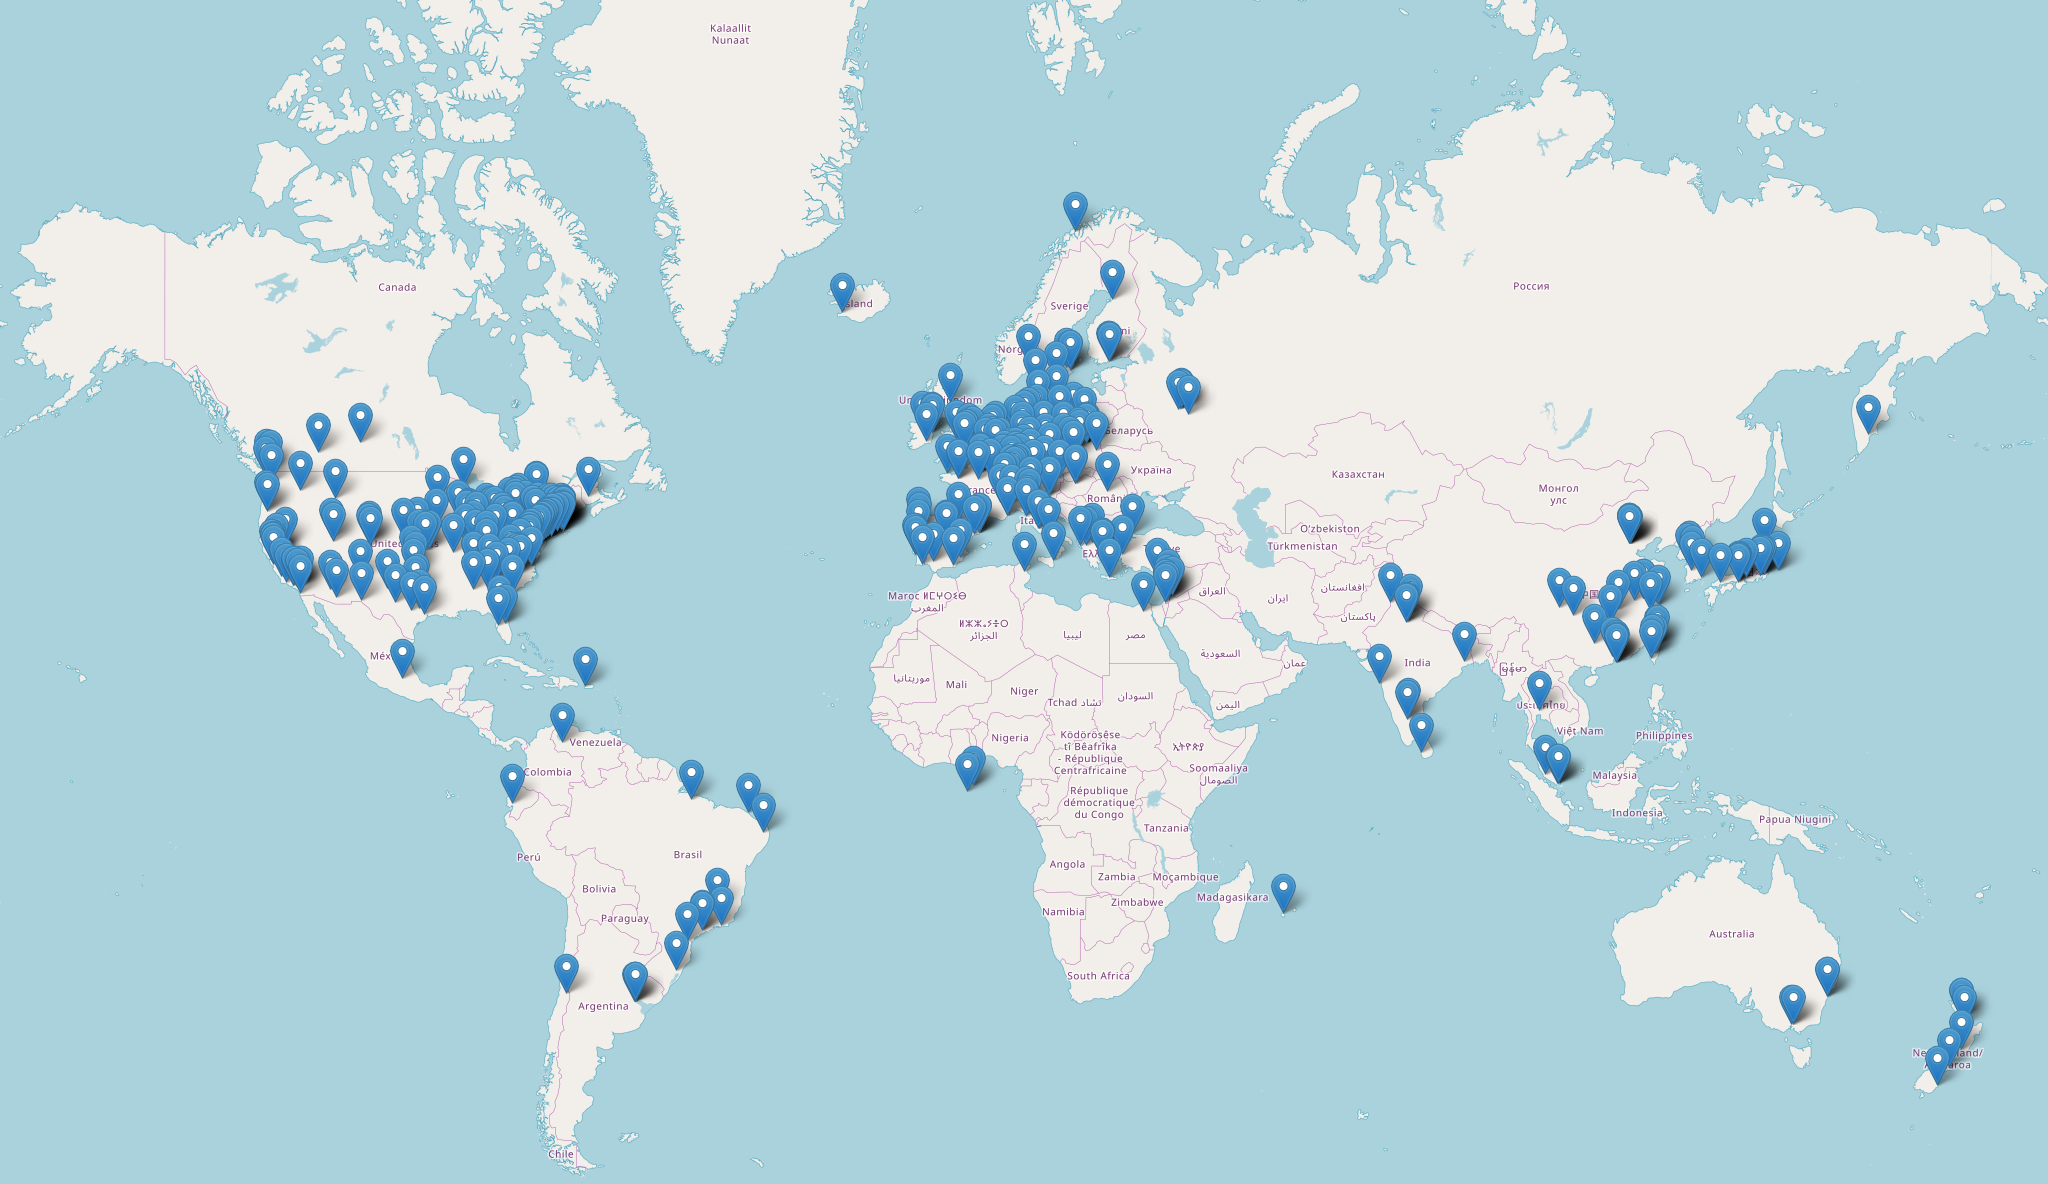
\includegraphics{obrazky/mapa_planetlab}}
	\caption{Map displaying location of the PlanetLab network nodes.}
	\label{fig:location}
\end{figure}

The tool's internal database created using PlanetLab \zk{zkAPI} (\zkratkatext{zkAPI}) consists of 1001 nodes which differs from the number described on the PlanetLab website and is most probably result of removing several nodes since the time website was updated. Important aspect to mention is that not all of those nodes are accessible. As shown in Figure~\ref{fig:pingablepie}, only 196 are responding to \zk{zkICMP} (\zkratkatext{zkICMP}) packets and 805 are not which is only around 19.58\% reponding nodes. That means 1.62\% nodes stopped responding since the last measurement done by Filip Šuba in his thesis \cite{suba1} in 2017. Important is to mention that this does not mean that the nodes are not accessible using \texttt{ssh} protocol. The \texttt{plbmng} tool can monitor accessibility of the nodes so its users always has overview which nodes can be actually used for their projects. The current committee of the project consists of members like Princeton University, Cambridge University, Intel, Google and many more \cite{planetlabmain}.\\

\begin{figure}[H]
	\centering
	\scalebox{0.6}{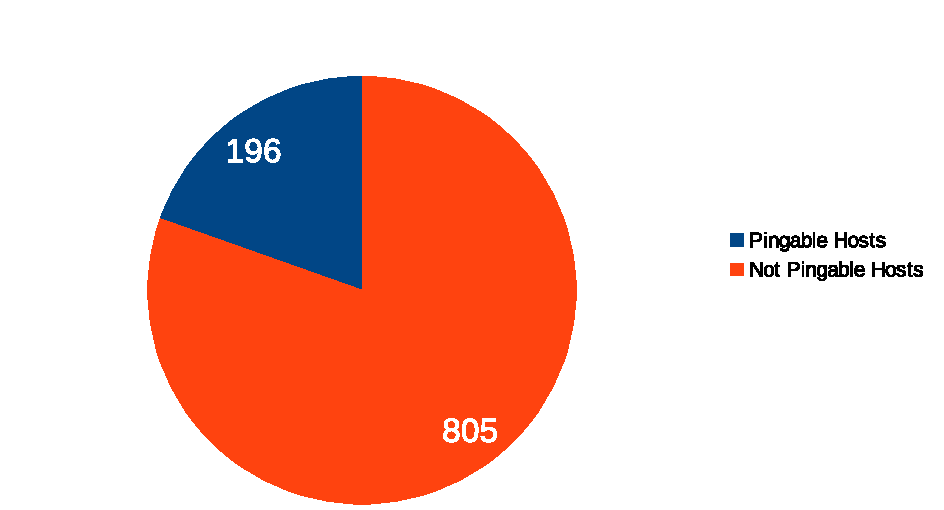
\includegraphics{obrazky/pingablepie}}
	\caption{Pie chart displaying number of nodes in PlanetLab network responding to ICMP packets.}
	\label{fig:pingablepie}
\end{figure}

\section{Terminology}
During the initial planning of \texttt{PlanetLab network} the authors agreed on using common terminology for aspects of the network and defined them in the \texttt{Phase 0 document} \cite{Roscoe_PDN-02-002} as follows:
\begin{itemize}
	\item \textbf{Node:} A~server machine capable of running components of PlanetLab services.
	\item \textbf{Site:} A~physical geographical location where PlanetLab nodes are located.
	\item \textbf{Cluster:} The set of PlanetLab nodes located at a given site.
	\item \textbf{User:} An authorized human being wishing to deploy or run service over PlanetLab network.
	\item \textbf{Client:} A~client of a service running over PlanetLab network.
	\item \textbf{Service:} An application running over PlanetLab network.
	\item \textbf{Application:} A~PlanetLab service not being part of PlanetLab infrastructure. 
	\item \textbf{Capsule:} A~component of a PlanetLab service that runs on a single node.
	\item \textbf{Slice:} A~distributed set of resources allocated to a service in PlanetLab.
\end{itemize}
\section{Selected Projects Based on PlanetLab}
In this section various projects that PlanetLab network enabled to create will be described. All these projects wouldn't be possible without the resources PlanetLab brings. On PlanetLab site there is partial bibliography of research enabled by PlanetLab and it consist of over two hundred projects \cite{planetlabmain}. Having over two hundred projects enabled by PlanetLab network shows that PlanetLab had succeeded in their initial goals which was to provide a useful platform for networking and system research \cite{Roscoe_PDN-02-002}. Example of projects enabled by PlanetLab are described in the following subsections.
\subsection{Securing Web Service by Automatic Robot Detection}
This project is focusing on detection of automatic robots by implementing a special form of Touring test. Detection is done by comparing human versus robot behavior on the websites. According to the authors, 95\% of the human users can be detected within the first 57 requests \cite{Park:2006:SWS:1267359.1267382}.
\subsection{The Design and Implementation of Next Generation Name Service for Internet}
Project that is aiming to solve the vulnerability of the current \zk{zkDNS} (\zkratkatext{zkDNS}) and slow delivery of updates to the system. Project paper describes design and implementation of the Cooperative Domain Name System (CoDoNS), a novel name service, which provides high lookup performance through proactive caching, resilience to denial of service attacks through automatic load-balancing, and fast propagation of updates \cite{Ramasubramanian:2004:DIN:1030194.1015504}.
\subsection{Slurpie: Cooperative Bulk Data Transfer Protocol}
Big data transfers can become problematic during peaks when huge amount of clients starts downloading the data at one point. This can occur for example during a launch of a new game or a new operating system. Slurpie is is a  a peer-to-peer protocol for bulk data transfer that aims to reduce client download times of large popular files and to reduce load on the providing servers \cite{1356981}. 

\chapter{Present State Of Application Development}
\label{chapter:plbmng}
Plbmng application, originally called \texttt{Data miner for PlanetLab}, is a supporting application for developing projects in the PlanetLab network. It gives its user an ability to discover and search PlanetLab servers, connect to them and upload or execute scripts. The tool is available at public PyPI repository\footnote{Link to PyPI repistory containing Data miner for PlanetLab tool: \url{https://pypi.org/project/plbmng/}}. The tool allows managing \texttt{PlanetLab} nodes, gathering information about them and pulling the latest data from the \texttt{PlanetLab} API service. Its core is written in Bash and additional modules are written in Python 3 \cite{suba1}. At the moment, it is depended on both Bash and Python modules and its installation consists of several steps:
\begin{itemize}
	\item Installing the application from PyPI repository or downloading the source codes from GitHub.
	\item Installing additional system packages like dialog,pssh and fping.
	\item Locating installation folder and putting symlink into \texttt{\$PATH} directory.
\end{itemize}
Since improvement of the installation process is in scope of this Semestral thesis, detailed post-improvement installation steps are described later in the Chapter~\ref{chapter:improve}.
\section{Description of Current Tool}
The tool consist of two layers. First one is the application logic layer and second one is graphical user interface layer, also known as menu, and consists of several options. First menu option is \texttt{Search nodes} for retrieving a node from internal database. This options allows user to either search by \zk{zkDNS} (\zkratkatext{zkDNS}), \zk{zkIP} (\zkratkatext{zkIP}) address or by node location. Second option is \texttt{Measure Menu} that allows user to schedule gathering of data about the nodes using \texttt{crontab}, select elements to monitor or start the data gathering right now. In the \texttt{Map Menu} option user has option to generate map showing location of the nodes and select map element. After the first start of the application, user is required to fill credentials and \texttt{SSH} public key details to be able to access \texttt{PlanetLab} API and nodes using the menu option \texttt{Settings}. Menu is created using bash library \texttt{dialog} and is shown in Figure~\ref{fig:planetlaboldmenu}. Graphical interface can be run directly in terminal making it available even through \texttt{ssh} client without setting up any graphical tools.

\begin{figure}[H]
	\centering
	\scalebox{0.5}{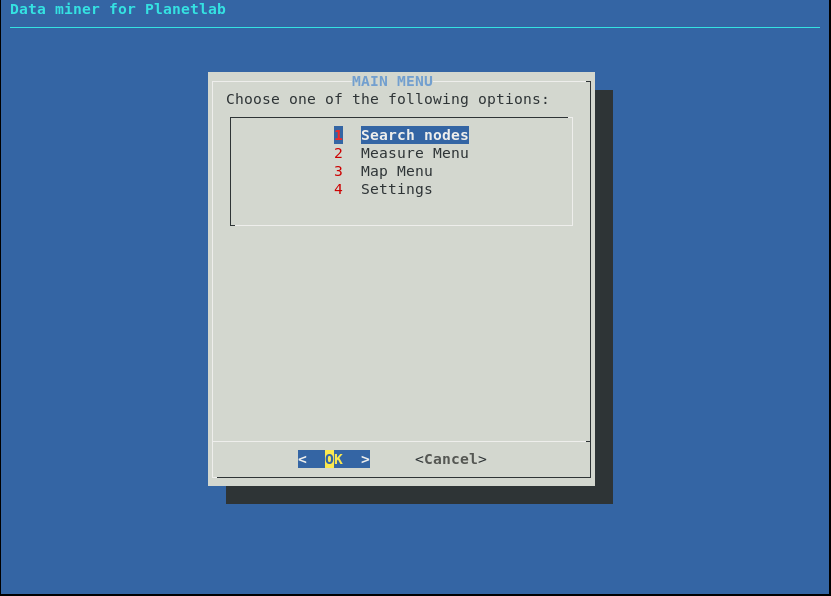
\includegraphics{obrazky/planetlabmenuold}}
	\caption{Data miner for PlanetLab menu.}
	\label{fig:planetlaboldmenu}
\end{figure}


\section{Current Problems}
\label{section:improvement}
The first problem of the existing tool is language disparity having half of the functionality in Bash and half of the functionality in Python 3. This makes it difficult to make adjustment to the tool as one needs to study a vast amount of scripts that are in several different folders. Since some of the functionality is done in Python 3, which is according to portal StackOverflow fastest-growing major programming language \cite{pythonfastestgrowing}, and because it is available at \zk{zkPYPI} (\zkratkatext{zkPYPI}), Python is an ideal candidate as a main language of the project. As a part of the Semestral thesis the existing code will be re-written into Python 3. Another great advantage of Python 3 is that it is multi-platform. As Mark Pilgrim mentions in his book \cite{Pilgrimc2010}, Python 3 is available on many platform such as \texttt{Windows}, \texttt{MacOS}, \texttt{Linux}, \texttt{BSD} and \texttt{Solaris} and their derivatives.\\
Second area of improvement is installation of the tool and post-installation steps. At the moment, it is required to install additional packages and tool is not automatically put into \texttt{\$PATH} folders forcing its users to locate the installation folder and run the script from there. Because of the single programming language being \texttt{Python 3} the dependencies for system packages will be removed and their \mbox{\texttt{Python 3}} counter-parts will be added as dependency for the PyPI package. PyPI installer takes care of these dependencies automatically during the installation procedure. To remove post-installation steps the tool will be written as library allowing to create a simple \texttt{Python} script in \texttt{bin} folder which is put into \texttt{\$PATH} folder by the PyPI installer during the installation.\\
Another improvement is renaming certain menu components and adding more information to the tool itself. This change is not significant and is purely cosmetic but can make it easier for new users to get familiar with the tool. The specific rename details will be later described in Subsection~\ref{subsection:readability}.\\
The tool currently contains a lot of bugs and bad coding practices. Example of a typical bug is whole application crashing because of missing file when returning back from \texttt{Search nodes} menu. During the rewriting into \texttt{Python 3} there is space to improve certain controls to avoid these crashes and needs to restart the application. As for bad code practices, as an example the tool currently calls functions recursively during returning from child menu page into parent one. This means the previous function menu is stored in the \texttt{stack} waiting for the application to end before released. During rewriting of the tool these implementation details can be changed to stick with the good coding practices. 

\chapter{Linux}
\label{chapter:Linux}
In this section the operating system Linux that PlanetLab nodes are running on, and that \texttt{plbmng} tool is developed for, will be reviewed and described. Operating system is a connecting layer between hardware and software. It provides interface to work with system resources such as disk, processor or memory and at the same time it provides service layer for client software to run at. Linux is an open-source operating system founded by Linus Torvalds who wrote its kernel using \texttt{C language} and began the history of Linux operating system. It was originally developed for personal computers based on the Intel x86 architecture but since its creation it has been ported to many other platforms such as mobile devices, television chips and many others. A~package containing Linux operating system is called Linux distribution. The defining component of each distribution is the Linux kernel \cite{eckert2012linux+}. Original Linux kernel has been created by Linus in 1991 \cite{linuxintro} and since them many other forks of this kernel has emerged. Some of the most famous are \texttt{Red Hat Enterprise Linux},  \texttt{CentOS}, \texttt{Fedora}, \texttt{Ubuntu},  \texttt{Debian} or \texttt{SUSE Linux}. More information about mentioned distributions can be found in at the end of this Chapter. The main advantages of Linux are:
\begin{itemize}
	\item Almost all Linux distribtuins are free and available for everyone.
	\item Linux is open-sourced and everyone can contribute and review what his/her machine is running.
	\item Linux can run on various platforms from personal computers to televisions.
	\item Linux is considered to be secure. Security model of Linux is based on UNIX security principals which are considered to be robust and verified \cite{BILHEQP2xqVnjbQi}. 
	\item Linux quickly adapt to changes. Since Linux has vast community behind it, it quickly adapt to security threads and new technologies.
\end{itemize}
On other hand, Linux has some disadvantages which will be summarized in the below list:
\begin{itemize}
	\item Requires more technical knowledge then other systems like \texttt{Windows} or \texttt{MacOS}.
	\item Huge amount of distributions can be confusing for new users to choose. 
	\item Many well known applications are primarily developed for \texttt{Windows} or \texttt{MacOS} (though many open source variants of these applications exists on Linux).
	\item Compatibility problems. Proprietary hardware can have issues with driver compatibility. Many hardware vendors are primarily focusing on \texttt{Windows} or \texttt{MacOS}.
\end{itemize}
asd\\
Linux kernel can be found in majority of devices at the moment. According to StatCounter Global Stats, 41.63\% of the machines are running on Linux kernel while 36.23\% are running on Windows-based kernel as of September 2018 \cite{StatCounter}. The rise of Linux kernel is conditioned by raising Android popularity and in 2016 the StatCounter states Linux kernel based system had only 28.44\% market share while Windows had 48.42\% market share \cite{StatCounter}. Linux can be found also in great amount of devices from phones, desktops, servers to television or cars. Server \texttt{opensource.com} states that more then half of all SmartTV devices runs on Linux \cite{opensourcecom}. Because Linux kernel is originally open-sourced, most of the devices worldwide runs on an open-sourced operating system which shows an interesting trend switching from proprietary software. In the following paragraphs, various popular Linux distributions will be described. Their key features will be reviewed and analyzed. 
\paragraph{Red Hat Enterprise Linux}
Red Hat Enterprise Linux is a Linux based distribution developed by Red Hat Inc. In 1994 the first version of Red Hat Linux has been released \cite{rhhistory}. Since it launch Red Hat became a popular enterprise Linux distribution and based on Red Hat's June 2017 statistic 100\% of all airlines, telcos and commercial banks in Fortune 500 runs on their software \cite{rhtrusted}. Red Hat advertise the system being robust and stable which is its biggest advantage for the enterprise companies. Even though Red Hat is open-sourced, it is not free as it is impossible to run it without having active subscription. Red Hat uses its own packaging system called \zk{zkYUM} (\zkratkatext{zkYUM}).
\paragraph{CentOS}
The \zk{zkCENTOS} (\zkratkatext{zkCENTOS}) is a Linux distribution that has been originally forked from Red Hat Enterprise Linux version 2.1 and released under name \texttt{CentOS-2} in May, 2014 \cite{centosfirsts} by John Newbigin. Since then it became a community-driven project that offers and free alternative to the Red Hat Enterprise Linux. Currently, CentOS Project is part of Red Hat while declaring to stay independent of the development of the Red Hat's Linux. Due to the distribution being free and for enterprises many companies and academic institutions choose the CentOS as the primary operating system for their servers.
\paragraph{Fedora}
Fedora is a Linux distribution developed by the communOriginally created in 1993 by Ian Murdock, Debian is a free Linux kernel based Unix like operating system developed by The Debian Project and its community. Debian in oposite to Red Hat Linux based systems uses different packaging system called \zk{zkAPT} (\zkratkatext{zkAPT}).ity and is sponsored by Red Hat. Currently, Fedora provides several types of system images such as Workstation, Server and Atomic. Fedora is distribution primarily used as a desktop operating system and shares many technologies with Red Hat Enterprise Linux and CentOS making packages compatible between these systems. Fedora is often considered to be somehow beta environment for changes before they make it to the more conservative Red Hat Enterprise Linux.
\paragraph{Debian}
Originally created in 1993 by Ian Murdock, Debian is a free Linux kernel based Unix like operating system developed by The Debian Project and its community. Debian in oposite to Red Hat Linux based systems uses different packaging system called \zk{zkAPT} (\zkratkatext{zkAPT}). In February 2016 the repositories of Debian consisted of 50007 binary packages \cite{debianfifty}. Debian is popular server distribution and in 2012 it was named by PCWorld magazine the most popular distribution for web servers \cite{debianpopular}.
\paragraph{Ubuntu}
Ubuntu is a free and open-source Linux distribution based on Debian operating system. It is being developed by 	Canonical and Ubuntu community. Currently Ubuntu offers three version of the system: Ubuntu Desktop for personal computers, Ubutnu Server for server and cloud and lastly Ubuntu Atomic created for \zk{zkIOT} (\zkratkatext{zkIOT}). It is seen that Ubuntu is making the Linux available for broader audience by having its graphical user interface more similar to other operating system like \texttt{MacOS} than other Linux distributions. Ubuntu also achieved great success when Microsoft ported official Ubuntu binaries into its Windows system. Ubuntu also is the most popular Linux distribution based on Google Trends data \cite{linuxtrends}.
\chapter{Virtualization}
\label{chapter:Virtualization}
Virtualization is an alternative to the traditional architecture. Comparison schema between virtualization and traditional architecture can be found in  Figure~\ref{fig:virtschema}. The traditional architecture consist of a hardware, operating system on the host and the applications running on it. The applications needs to be compatible with the operating system to be able to run on it. On the other hand, virtualization is a layer over the hosting operating system and offers an interface for the guest operating system to use by emulating various resources such as disk, network usb and many more. Guest operating system are operating systems of the virtual hosts running on the hypervisor. Hypervisor is providing resources to each virtual host. This enables better resource handling since all the virtual machines share same resources and theoretically have access to much higher computing power. Another advantage is backward compatibility as various operating systems of a kind can be running one one host. Example is legacy version of a system that is no more compatible with current hardware but is compatible with the virtualization software. This can be particular useful for institutions that requires extremely stable well tested software running on legacy system. Next feature is high availability. If a virtual host crashes, many virtualization software are capable to migrate the run-time data to another virtual host live time. This can be crucial feature for any critical applications. On bare-metal hosts this can be solved by using for example clustered hosts.\\

\begin{figure}[H]
	\centering
	\scalebox{0.7}{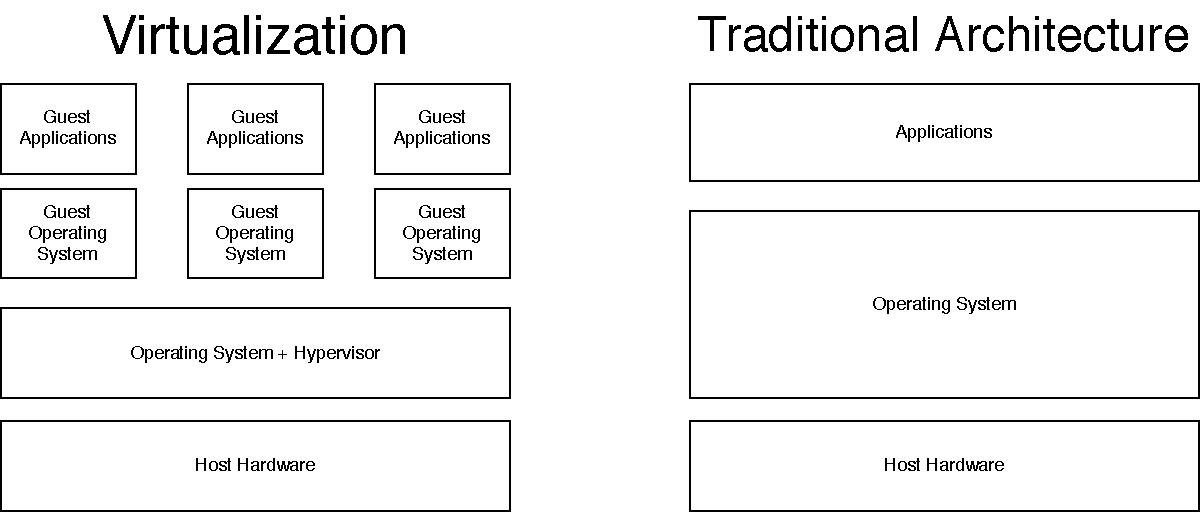
\includegraphics{obrazky/virt}}
	\caption{Virtualization vs traditional architecture schema.}
	\label{fig:virtschema}
\end{figure}

Currently there are many virtualization technologies available on the market. Some of the most popular ones are \texttt{VMware ESXi}, \texttt{Red Hat Enterprise Virtualization}, \texttt{Oracle Virtualbox} and \texttt{QEMU/KVM} \cite{virtualizationpopular}. In the following lines, some of the most popular Virtualization technologies are reviewed.
\paragraph{VMware ESXi}
VMware is a company providing virtualization software. The company provides several versions of virtualization software including \texttt{VMware ESXi} which is an enterprise virtualization solution. \texttt{VMware ESXi} was developed to run directly on the bare-metal hardware and doesn't require any other operating system to be installed on the host as it uses its own operating system called VMkernel \cite{vmwarearch}. This allows the software direct access to the hardware as it includes its own vital OS components. As VMware states in their architecture document \cite{vmwarearch}, this also allows better hypervisor security, increased reliability,
and simplified management. 
\paragraph{Red Hat Enterprise Virtualization}
As Red Hat states on their website, \texttt{Red Hat Enterprise Virtualization} is an open, software-defined platform that virtualizes Linux and Microsoft Windows workloads \cite{rhev}. \texttt{Red Hat Enterprise Virtualization} is a software that is developed to run on Red Hat Enterprise Linux, a Linux distribution developed by the same company. As Red Hat states in \texttt{Red Hat Enterprise Virtualization} datasheet, the biggest advantage of the software is its integration with other \texttt{Red Hat} products \cite{rhdatasheet}. Red Hat also offers a complete operating system designed for creating virtual machines called \texttt{Red Hat Enterprise Virtualization Hypervisor}.
\paragraph{Oracle Virtualbox}
\texttt{Oracle Virtualbox} is open source virtualization software available for both enterprise as well as home use and is developed by Oracle Corporation. As stated on the Oracle Virtualbox website: "Presently, VirtualBox runs on Windows, Linux, Macintosh, and Solaris hosts and supports a large number of guest operating systems including but not limited to Windows (NT 4.0, 2000, XP, Server 2003, Vista, Windows 7, Windows 8, Windows 10), DOS/Windows 3.x, Linux (2.4, 2.6, 3.x and 4.x), Solaris and OpenSolaris, OS/2, and OpenBSD." \cite{oraclehome} which is a considerable availability. \texttt{Oracle Virtualbox} offers many features, which are more described in the User Manual \cite{oracledatasheet}, such as:
\begin{itemize}
	\item VBoxManage, a command-line interface for \texttt{Oracle Virtualbox}.
	\item No hardware virtualization required, supporting even older hardware without build-in virtualization support. 
	\item Guest Additions, which is a software packages that offers features like folder sharing, automatic window focus, 3D virtualization and more.
	\item Multigeneration branched snapshots, which allows taking snapshot of the virtual host in any point of time completely saving the machine state allowing users to later revert machine to the saved state.
\end{itemize}
\paragraph{KVM with QEMU}
\zk{zkKVM} (\zkratkatext{zkKVM}) is a kernel module that provides a \zk{zkCPU} (\zkratkatext{zkCPU}) virtualization through the use of Intel VT or AMD-V hardware extensions. KVM runs in kernel space and handles elements like processor switching or \zk{zkMMU} (\zkratkatext{zkMMU}) registers, which are used to handle the virtual machines. On the other hand, QEMU is a free open source emulator that performs hardware virtualization in the user space part of the operating system. On its own, QEMU provides also CPU emulation through binary translation however the best results are delivered when combined with KVM and it can deliver near native performance \cite{kvmspeed}. During measurement of virtual machine versus host performance using the KVM technology the Geekbench’s GPU test shown only 1.19\% score decrease over the bare-metal host \cite{kvmbenchmark}.


%% Vložení souboru 'text/vysledky' s popisem vysledků práce
\chapter{Implemented Improvements to PlanetLab Server Manager}
\label{chapter:improve}
This Chapter will discuss improvements made to the PlanetLab application. The improvements are based on the analysis made in the Section~\ref{section:improvement}. The implementation details will be described and shown. The goal of the re-implementation is to make the \texttt{plmbng} tool simple to use, easier to contribute into by re-writing it fully into Python~3, using good coding practices, remove any post-installations steps and making small improvements. Improvements includes:
\begin{itemize}
	\item Removing result limitation by dynamically creating menu using Python \texttt{list}.
	\item Adding support to use application as library by logically separating each function.
	\item Increasing readability and improve orientation in the application by renaming menu components and using descriptive functions names.
	\item Eliminating pre and post installation steps by using automatic \texttt{pip} dependency installer.
	\item Improving credentials set up by adding internal text editor.
	\item Extending Windows support to several functions by detecting operating system and dynamically changing parameters.
	\item Adding filtering option to limit search of nodes based on their availability.
	\item Displaying last accessed server.
	\item Adding information about nodes on a~map.
	\item Adding status menu option to show latest statistics using internal database.
	\item Several bug fixes and other minor improvements.
\end{itemize}

\section{Re-design of Application}
\label{section:redesign}
This Section will describe the approach taken to improve the application. The issues of the application, described more in Section~\ref{section:improvement}, are that there are two different languages, functions are scattered and application folder structure is confusing. During re-design, all these problems were taken into consideration and addressed. First problem, already well described, was solved by re-writing the application fully into Python~3 language. Second and third problem were resolved by re-designing the application folder structure and architecture. The overall architecture of re-designed application is shown in Figure~\ref{fig:archdiagram} and will be described in the next paragraph.\\

\begin{figure}[H]
	\centering
	\scalebox{0.8}{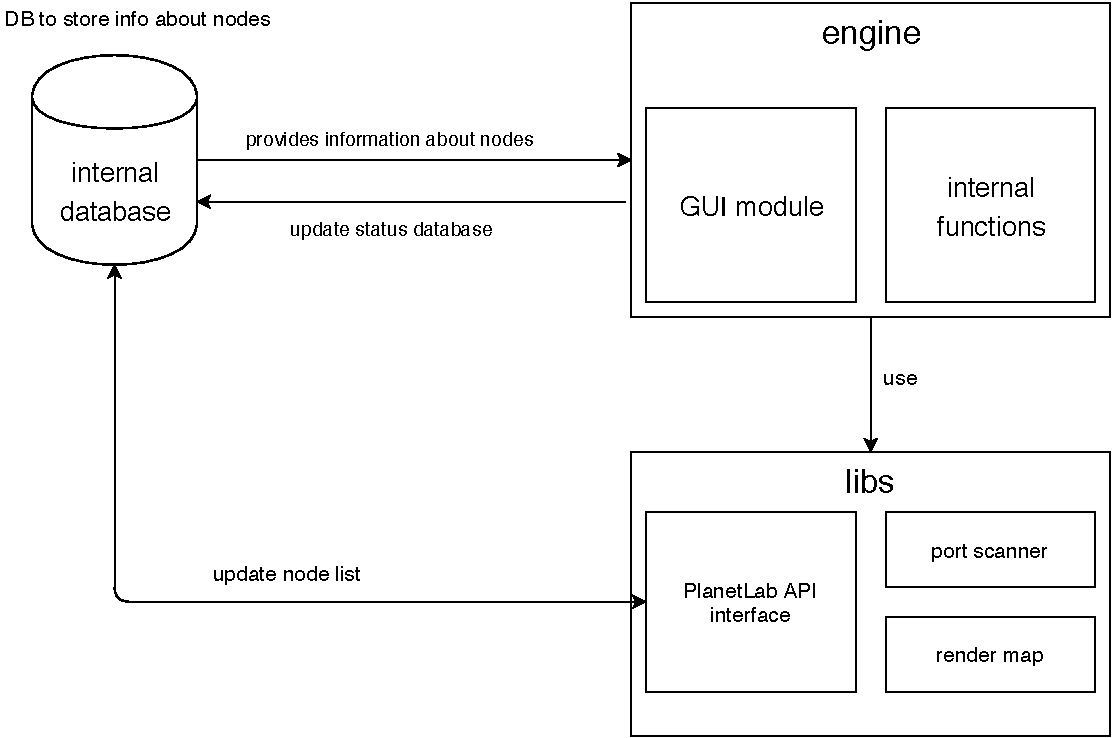
\includegraphics{obrazky/PlbmngArchitecture}}
	\caption{New PlanetLab Server Manager architecture diagram.}
	\label{fig:archdiagram}
\end{figure}

Issue with scattered functions was solved using single file, the \texttt{engine.py}, for all the common internal functions and graphic functions and libraries for more complex functionality of the application. To make it easier to navigate inside the engine file, it was divided between graphic and internal logic sections. A~question why not to split the graphical and internal logic might come to a~mind. Currently, the engine module graphical and internal functions are calling each other as an reaction to certain states. Splitting them would mean importing each other in a~circle which is not an ideal state. Having both sections in one file makes it one solid logical component, called the engine. However as mentioned, there are certain independent components that are split into their own files. In the Figure~\ref{fig:archdiagram}, these are described as \texttt{libs} and contains several utility functions that can be called independently and are imported as a~library inside the \texttt{engine}. Currently, there are three of these utility modules. PlanetLab API interface, which provides data~for updating the application database of servers, port scanner which allows to check port accessibility of remote host and lastly module that allows to render map of nodes using a~dictionary of nodes as input. On of the challenges during re-design was a~placeholder for all the information about nodes that application can later used. Previously, a~text file was used to store this data. Issue with this is to implement a~filter function for example, it would require to write a~custom module for queries which is an unnecessary overhead as there are already solutions available to provide such module. One of these solution is relational database with SQL used as a~query language. SQL is a~structured query language designed to manipulate data~in relational tables which are nothing more than set of related information~\cite{Beaulieu:2005:LS:1098720}. This fits perfectly application needs as it stores a~set of nodes with their related status information. In the Figure~\ref{fig:archdiagram}, this is shown as an internal database module. Engine triggers update of status of available nodes whereas PlanetLab API interface library updates the list of nodes. Python provides a~\texttt{SQLite3} library that allows creating a~custom database stored on disk. This database file is placed inside the database folder in the application configuration management. Mentioned architecture decisions will allow application to be more easily salable and maintainable in the later development phases.\\

\section{Description of Improvements}
\label{section:implementapproach}
In this Section, the steps to achieve goals--which were described in the Chapter introduction--will be shown in detail in their own Subsections. For each Subsection the approach, specific steps, code examples and results will be illustrated. Since the new implementation uses \texttt{pythondialog} module, at the start of the tool an instance of the \texttt{Dialog} class is spawned and will be later described just as the \texttt{instance}.
\subsection{Removal of Search Result Limitation}
The previous version of \texttt{plbmng} tool has been limited to 10 result while searching for a~node. This issue was introduced due to difficulty of creating a~menu based on dynamic results since author needed to always append another argument to the overall menu command. This approach can also hit limitation of characters that can be passed in a~Bash command line. In Python~3 this problem does not exists since \texttt{pythondialog} module is creating menu functions based on \texttt{list}. During the search of nodes, results are added to the list which is after completed search passed to the instance which renders the \zk{zkGUI} (\zkratkatext{zkGUI}). Example of this functionality is shown in Listing~\ref{lst:removingresultlimit}. Due to this improvement tool is returning all results found.

{\noindent\begin{minipage}{\linewidth}
\begin{lstlisting}[language=Python, numbers=left, label={lst:removingresultlimit}, caption=Removing result limitation by passing choices as a~list argument., frame=single, showstringspaces=false, keywordstyle=\color{blue},captionpos=b]
def searchNodesGui(prepared_choices):
	if not prepared_choices:
		d.msgbox("No results found.", width=0,height=0)
		return None
	while True:
		code, tag = d.menu("These are the results:",
							choices=prepared_choices,
							title="Search results")
\end{lstlisting}
\end{minipage}

\subsection{Writing the Application as Library}
For the application to be used in other scripts and to reduce need to re-write certain code parts it is desired to write application to be able to run as a~library. During the re-implementation this was considered and application is available both as library and standalone script. This will be later used in the Subsection~\ref{section:improvement}. If the application is called as a~standalone script it will trigger part of the code that is shown in Listings~\ref{lst:pythoninit} which will initialize graphical interface. If imported as a~library, it allows the user to call any function defined in the script.

{\noindent\begin{minipage}{\linewidth}
\begin{lstlisting}[language=Python, numbers=left, label={lst:pythoninit}, caption=Condition to recognize that application is being called as a~standalone script., frame=single, showstringspaces=false, breaklines=true, keywordstyle=\color{blue},captionpos=b]
if __name__ == "__main__":
	initInterface()
	exit(0)
\end{lstlisting}
\end{minipage}

\subsection{Code Readability Improvement}
\label{subsection:readability}
Community is a~powerful group that helps develop a~tool and to add more functionality to it. To have community contribute to a~tool, it should follow good practices and be easily readable and understandable. Previous version of the tool was using Bash script which was calling Python script and creating new Bash scripts on a~disk which was merging using different pieces of code from pre-created \texttt{.dat} files in a~\texttt{bin} folder. Finding a~bug in this structure was difficult and navigating was not intuitive. Most functions were fully re-written into single Python script and logically divided into two sections. One section is for GUI functions and other is for logical functions. Stand-alone functions were moved to a~separated scripts to be used as a~library. Each functions is very descriptive in its name as shown in Listing~\ref{lst:descriptive}.

{\noindent\begin{minipage}{\linewidth}
\begin{lstlisting}[language=Python, numbers=left, label={lst:descriptive}, caption=Example of Function Names, frame=single, showstringspaces=false, breaklines=true, keywordstyle=\color{blue},captionpos=b]
def searchNodes(option,regex=None):
def initInterface():
def plotServersOnMap(mode):
def getPasswd():
def searchNodesGui(prepared_choices):
def printServerInfo(chosenOne):
def setCredentialsGui():
\end{lstlisting}
\end{minipage}

Each functions is trying to be as atomic as possible only having one purpose. This is helping to increase modularity of the application. Outside of this function "categories" tool is removing any \texttt{magic numbers} by defining constants at the beginning of the source code. This greatly helps to understand what is being passed as an argument and is shown in Listing~\ref{lst:constant} where it is descriptive what option is being passed as a~search key to the \texttt{searchNodes} function. Also, the application has a~block for \texttt{Initial settings} at the beginning for one single place where outside of functions definitions can be placed. Application is also honoring the conventions defined in \zk{zkPEP} (\zkratkatext{zkPEP}) 8 \cite{pythonpep}, like naming convention and space usage instead of tabs, as much as possible. In default, scripts like \texttt{pylint} uses snake case style naming convention however camel case that is actually described in the official pep 8 standards as a~recommended descriptive naming style \cite{pythonpep}. All these small items described are increasing the overall readability of the application for others to quickly become familiarized with it. Currently, main script \texttt{engine.py} received score of 7.38  \texttt{pylint} with main complains being about missing doc strings and certain minor warnings regarding wrong import and other small deviation from the PEP 8 standard.

{\noindent\begin{minipage}{\linewidth}
\begin{lstlisting}[language=Python, numbers=left, label={lst:constant}, caption=Example of Constant Usage, frame=single, showstringspaces=false, breaklines=true, keywordstyle=\color{blue},captionpos=b]
code, tag = d.menu("Choose one of the following options:",
					choices=[("1", "Serach by DNS"),
				      		 ("2", "Search by IP"),
					    	   ("3", "Search by location")],
						       title="ACCESS SERVERS")
if code == d.OK:
	#Search by DNS
	if(tag == "1"):
		code, answer = d.inputbox("Search for:",title="Search")
		if code == d.OK:
			searchNodes(OPTION_DNS,answer)
		else:
			continue
\end{lstlisting}
\end{minipage}

As mentioned in the Section~\ref{section:improvement}, renaming certain parts of the tool can improve the readability. Since the tool is not data~mining rather than server manager, the tool is renamed from \texttt{Data~miner or PlanetLab} into \texttt{PlanetLab Server Manager}. Version is added next to the name for users to see which they are running immediately. Another example is renaming \texttt{Search nodes} to \texttt{Access servers} since primary function of this menu item is to access the servers while search is just supporting it. The re-designed application can be seen in Figure~\ref{fig:redesigned}.\\

\begin{figure}[H]
	\centering
	\scalebox{0.58}{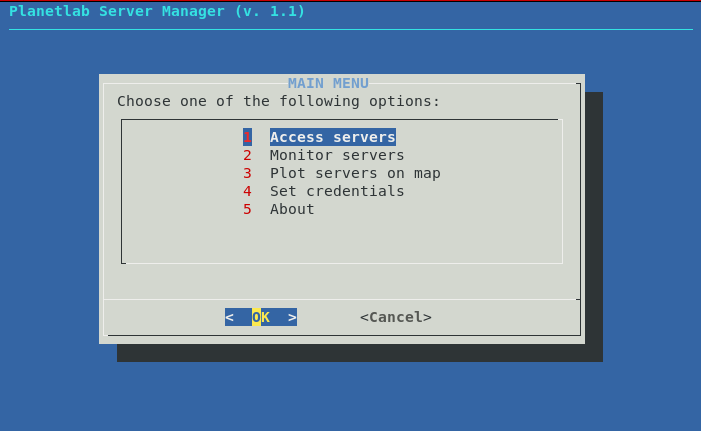
\includegraphics{obrazky/plbmng_basic}}
	\caption{Re-designed menu of new PlanetLab Server Manager.}
	\label{fig:redesigned}
\end{figure}

\subsection{Removal of Pre and Post Installation Steps}
Previous version of application required several pre and post installation steps. In the new version developed as part of this Diploma~thesis, all these steps were removed. Pre-installation steps were eliminated by completely getting rid of dependencies on additional system packages. All dependencies were moved into the PyPI package definition and are taken care off PyPI installer during installation of the tool. Post-installation steps were removed by adding the application into \texttt{bin} folder in the PyPI package. During installation, the PyPI installer automatically puts any scripts in the \texttt{bin} folder into a~\texttt{\$PATH} folder making it accessible directly from command line without the need of accessing installation folder. The contents of the main, but simple, script located in \texttt{bin} folder can be seen in Listing~\ref{lst:plbmngbin}.

{\noindent\begin{minipage}{\linewidth}
\begin{lstlisting}[language=Python, numbers=left, label={lst:plbmngbin}, caption=Source code of the main script populated by PyPI installer into executable folders., frame=single, showstringspaces=false, breaklines=true, keywordstyle=\color{blue},captionpos=b]
#! /usr/bin/env python3
from plbmng import engine
import sys

if len(sys.argv) > 1:
	if(str(sys.argv[1]) == 'crontab'):
		engine.updateAvailabilityDatabaseParent('cron')
		exit(0)

engine.initInterface()
\end{lstlisting}
\end{minipage}}

\subsection{Improvement of Credentials Management}
In the previous version of the tool the credentials were filled using \texttt{dialog} forms. When typing the credentials, nothing was shown except stars thus user was unaware where is the position of the cursor. Also saving the credentials was not working properly resulting into the need to adjust the configuration file on the disk which required locating the file first by inspecting the source code. In the new version settings credential is improved by creating a~virtual editor in the graphical interface itself, as shown in Figure~\ref{fig:credentials}, which allows the user transparently set the credentials. One of the disadvantage of this approach is plain text visible password in the editor as it is not hidden and user needs to be careful about setting the credentials in a~safe environment. To the addition of this improvement, various credentials checks were added to the application. First run of the tool will always trigger pop-up window advising user to fill credentials first. If a~user chose to update a~database without having credentials filled a~warning message will pop-up warning the user about that fact. Also, when user wants to ssh to a~server without having username and key filled he will have warning text near the ssh option. These improvements should prevent users forgetting about filling credentials and failing actions in the application.

\begin{figure}[H]
	\centering
	\scalebox{0.5}{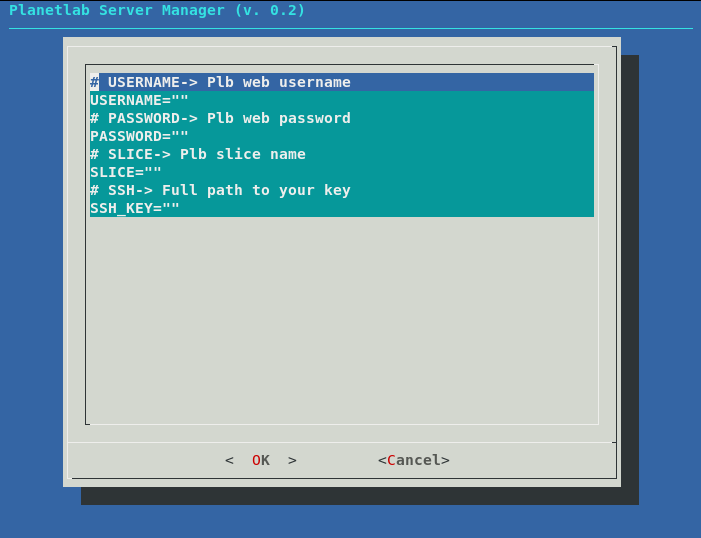
\includegraphics{obrazky/credentials_figure}}
	\caption{New window for setting up credentials using internal text editor.}
	\label{fig:credentials}
\end{figure}

\subsection{Application Folder Structure Re-design}
With changes to the architecture of the application, folder management needs to be also adjusted accordingly. The root folder of the application contains two main parts, outside of necessary PyPI files. It is the \texttt{bin} folder with \texttt{plbmng} script itself and the \texttt{plbmng} folder which contains the whole application logic and graphical interface. This folder will be now described in detail. As characterized in Section~\ref{section:redesign}, libraries are placed in the \texttt{lib} folder instead of \texttt{python\_scripts} previously. In past, the configuration files were stored in \texttt{bin} folder with shell scripts. This has been re-named to \texttt{conf} folder and library functions were moved to the \texttt{lib} folder. There are information that needs to be stored persistently, like information about accessibility of nodes. For this purposes, there is a~folder called \texttt{database} which contains file like \texttt{internal.db} which is already mentioned \texttt{SQLite3} database. With all these changes to the folder structure, the project should be now more transparent, clear and easier for other developers to join the project.

\subsection{Filtering Nodes Based on Accessibility}
One of the goals if this Diploma~thesis was to add a~functionality to filter nodes based on their accessibility. This Subsection will describe how the functionality was designed and implemented. The overall idea~was to add a~way to filter current node based on their availability, have an option to change these settings, show these settings and have a~way to update the data. In the following paragraph, all these items will be described more in detail.\\
As it was mentioned in Section~\ref{section:redesign}, the core of this functionality was to have a~placeholder for the data~about the nodes. This was achieved using the \texttt{SQLite3} Python library. To store the information, table \texttt{availability} was created and its structure can be seen in Table~\ref{table:availability}. First, \texttt{nkey} column is a~primary key column that contains ID of the table row. Next is \texttt{shash} that contains unique hash of the node hostname. This hash is used to find already existing records so these are not duplicated but only updated. Hash is generated using md5 function and \texttt{hashlib} Python library. Next column is a~\texttt{hostname} of the node for purposes of filtering and lastly there is the double \texttt{bssh} and \texttt{bping} which are Boolean flag displaying node accessibility. During insert into the database, \texttt{nkey} is automatically incremented thus only other values needs to be specified. Before the filtering is explained, first the internal logic working with nodes needs to be characterized. When an user select to display nodes, the search function takes a~dictionary of nodes as an input parameter. This simple logic is used for the filtering itself. In the function \texttt{getNodes()}, before the list of nodes is parsed, the current settings are loaded from the database from the \texttt{configuration} table which contains simply ID, name of the setting and Boolean if it is enabled or not. These settings are used to get all hostnames of the nodes that fits the current settings. For example, if user wants to filter only ssh available nodes, the query will be \texttt{select * from availability where bssh='T'}. With the list of desired nodes the function will always return only nodes that fits user's filter criteria.\\

\begin{table}[htb]
	\resizebox{\textwidth}{!}{\begin{tabular}{|l|l|l|l|l|}
			\hline
			\rowcolor[HTML]{EFEFEF} 
			nkey & shash                            & shostname                                & bssh & bping \\ \hline
			2    & fe27ca7d1707e86e1739b1819743dc79 & planetlab2.fri.uni-lj.si                 & F    & F     \\ \hline
			3    & 57da801bf4370f2a163a81bdf6bafa8c & ple01.fc.univie.ac.at                    & T    & F     \\ \hline
			4    & 3c956d5e295f17cb303773f83c84bf17 & aladdin.planetlab.extranet.uni-passau.de & T    & T     \\ \hline
		\end{tabular}
	}
\centering
\caption{Structure and examples of availability table for filtering functionality.}
\label{table:availability}
\end{table}

Applying filters is done using \texttt{Filtering options} in the \texttt{Access servers} menu. As shown in Figure~\ref{fig:filtering}, user can choose between ssh or ping available nodes. The selection is done using checkboxes. The choices are then shown in the  \texttt{Access servers} menu on the top as \textit{Active filters} line with the listing of the active options. \\

\begin{figure}[H]
	\centering
	\scalebox{1}{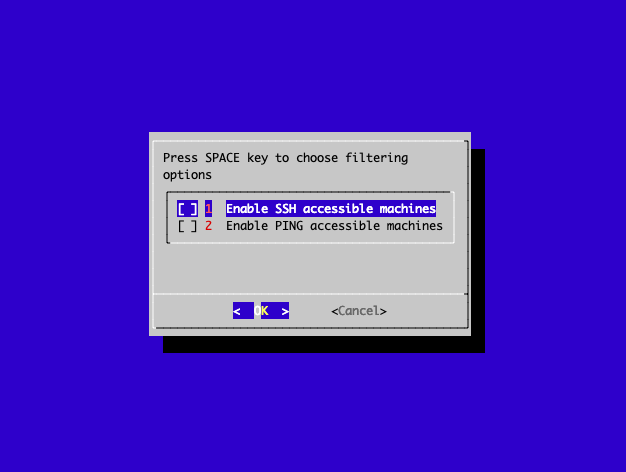
\includegraphics{obrazky/filtering}}
	\caption{Figure showing new menu where user can choose active filters.}
	\label{fig:filtering}
\end{figure}

\subsection{Multiprocessing Update of Status Database}
Updating the status database, or to be precise updating table inside the database, can be triggered from the \texttt{Monitor servers} menu. This will start a~progress bar that takes approximately two minutes after optimization. Before optimization, the procedure took around 40 minutes. This speed was reached using multi-processing. Once procedure to update database is triggered, fifty processes are spawned at a~same time using Python \textit{multiprocessing} library. List of nodes is passed as an iterator to go over in a~loop to the \texttt{Pool} object as shown in Listing~\ref{lst:multiprocess}. In addition, one lock is created to take over critical section of updating the shared status database and progress bar. Critical section can be defined as an area~in a~computer program where process operates on the shared variable by changes its value \cite{gebali2011algorithms}. Once a~process reaches the critical section, it needs to acquire the lock to enter into it. Once a~process has acquired the lock, it can start writing into the shared memory without any issue. As soon as it is done, the lock is released and another process can acquire it and start writing into the critical section. To be able to show correctly the progress, once a~process finishes a~task, it will lock the progress bar value, increase the progress variable with an increment that is derived from total number of nodes and then unlock the progress bar iterating to another node to gather information about it. The code of entering the critical section can be seen in  Listing~\ref{lst:lock}\\
 
{\noindent\begin{minipage}{\linewidth}
		\begin{lstlisting}[language=Python, numbers=left, label={lst:multiprocess}, caption={Creating a~multi-processing object with fifty processes, three shared variables and list of nodes as iterator.}, frame=single, showstringspaces=false, breaklines=true, keywordstyle=\color{blue},captionpos=b]
pool = Pool(50, initializer=multiProcessingInit,
		  	initargs=(lock,base,increment, ))
pool.map(updateAvailabilityDatabase, nodes)
		\end{lstlisting}
	\end{minipage} 

{\noindent\begin{minipage}{\linewidth}
		\begin{lstlisting}[language=Python, numbers=left, label={lst:lock}, caption=Entering a~critical section and acquiring lock., frame=single, showstringspaces=false, breaklines=true, keywordstyle=\color{blue},captionpos=b]
lock.acquire()
base.value = base.value = increment.value
updateProgressBarMultiProcessing(base.value)
lock.release()
		\end{lstlisting}
	\end{minipage} 

\subsection{Improvements of Node Visualization}
In the previous version of the application, user could render all nodes in the node database on a~map. It displayed markers which, upon clicking, showed hostname of the node. During implementation of filters, maps were also enhanced. Now, user can select between three maps to render; full map, map of nodes available over ssh and map of nodes that are ping-able. In addition, upon clicking, user can see all the stored information about the node as can be seen in Figure~\ref{fig:mapnodedetail}. The library for rendering the map was changed to use the same principle as search function. Instead of reading nodes from a~file, it gets them passed as a~parameter. While triggering the map module, nodes are loaded using \texttt{getNodes()} function that takes filtering into consideration in default. The filter in this case is only adjusted by the user's choice. Later, in Section~\ref{section:analysis} the information from map filters will be used to analyze \textit{PlanetLab Network} more in detail. For user, maps filters are good opportunity to see which server are actually available for project testing and possibly create an uniform list of candidate nodes that are spread all over the world. 

\begin{figure}[H]
	\centering
	\scalebox{0.65}{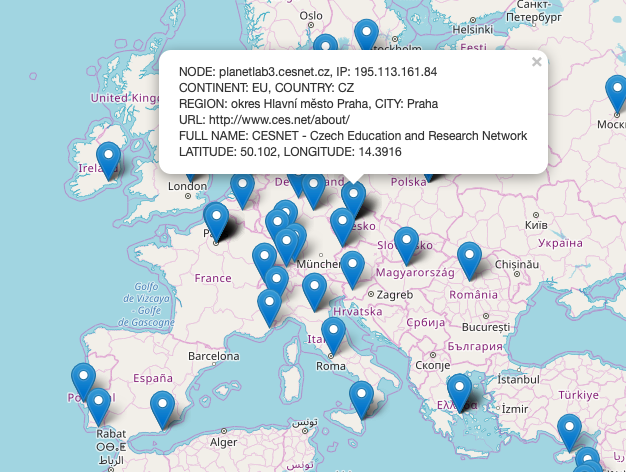
\includegraphics{obrazky/mapnodedetail}}
	\caption{Detail of node marker with newly added information about the particular node \cite{OpenStreetMap}.}
	\label{fig:mapnodedetail}
\end{figure}

\subsection{Minor Improvements}
In this Subsection, minor improvements done during the re-implementation are described. All these improvements were considered minor hence they do not have separate Subsection.
\paragraph{Clearing of the screen after cancel}
When signal was send to the application using \texttt{CTRL + C} key combination, the previous version of the application was not clearing the current terminal window and the GUI. To use the same terminal user was forced to clear the window manually. In the new version, when signal is send to the application, signal handler will catch it and clean after itself.
\paragraph{Recursion removal for return}
When returning from child window to a~parent page, the previous version of application was recursively calling the GUI function. This is not following good coding habits as each recursive call means storing the previous function details into the system stack, unnecessarily filling it. In the new version, while cycle is used instead and returning from a~function results into new iteration of the while cycle not storing anything onto the system stack. 
\paragraph{About is added to the menu}
About section is added to the menu displaying version, authors and the license.
\paragraph{Crontab mode created}
Application has option to run with \texttt{crontab} argument which will trigger just monitoring of the nodes. This is in particular useful when setting the \texttt{crontab} since the call can be simply \texttt{plbmng crontab}. This mode can be used to setup a~regular updates in background to the node database.
\paragraph{Last server access}
User has now ability to return to last accessed server it the \texttt{Access servers} menu. In default, this option will just print warning message that no node was accessed. However, as soon as user access first node, this node is stored into the database in form of dump of the node dictionary variable. If user wants to access the last accessed node, this dictionary is dumped back to an internal variable and used to show this node with all the information and options.
\paragraph{Menu with statistics}
Since status database already contains all the necessary information a~simple functionality regarding accessibility of the stored nodes was added to the application as can be seen in Figure~\ref{fig:statmenu}. 

\begin{figure}[H]
	\centering
	\scalebox{1}{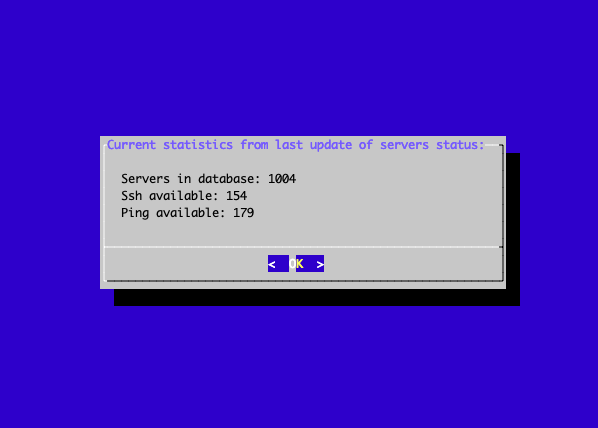
\includegraphics{obrazky/statmenu}}
	\caption{Newly added option to display current statistics about accessibility of stored nodes.}
	\label{fig:statmenu}
\end{figure}

\paragraph{Support of Multiple Platforms}
As was mentioned previously, Python is multi-platform language and brings possibility of porting the application to all kinds of different operating systems. During the re-implementation of the application this was taken into considerations and new functions were written to be able to run on Linux, Mac and possibly later on even Windows. Example of this multi-platform implementation can be seen in Listing~\ref{lst:testping} showing function \texttt{testPing} supporting all mentioned operating systems. As both Linux and Mac are Unix based, the implementation for these operating system is fairly simple and only minor changes are usually in several parameters. Good example is \texttt{ping} function. On Mac, time-out parameter takes one integer in millisecond as input variable. However, on Linux, the time-out parameter takes the integer variable in seconds. These little differences needs to be kept in mind when implementing platform-based functions. For Windows however, the differences are even more complex and all the libraries used in \texttt{plbmng} have to have Windows support. This was never tested yet even though most of the functions were written with Windows in mind. Adding full Windows support is a~good initiative for the future development of \texttt{plbmng}.

{\noindent\begin{minipage}{\linewidth}
		\begin{lstlisting}[language=Python, numbers=left, label={lst:testping}, caption={Example of fully multi-platform function testPing.}, frame=single, showstringspaces=false, breaklines=true, keywordstyle=\color{blue},captionpos=b]
def testPing(target, returnbool=False):
	pingPacketWaitTime = None
	if system().lower() == 'windows':
		pingParam = '-n'
	else:
		pingParam = '-c'
	#for Linux ping parameter takes seconds while MAC OS ping takes miliseconds
	if system().lower() == 'linux':
		pingPacketWaitTime = 1
	else:
		pingPacketWaitTime = 800
	command = ['ping', pingParam, '1', target, '-W', str(pingPacketWaitTime)]
	p = subprocess.Popen(command, stdout=subprocess.PIPE,
	stderr=subprocess.PIPE)
	# prepare the regular expression to get time
	if system().lower() == 'windows':
		avg = re.compile('Average = ([0-9]+)ms')
	else:
		avg = re.compile(
		'min/avg/max/[a-z]+ = [0-9.]+/([0-9.]+)/[0-9.]+/[0-9.]+')
		avgStr = avg.findall(str(p.communicate()[0]))
	if p.returncode != 0:
		if not returnbool:
			return "Not reachable via~ICMP"
		return False
	else:
		p.kill()
		if not returnbool:
			return avgStr[0]+" ms"
		return True
		\end{lstlisting}
	\end{minipage}

\subsection{Minor Bug Fixes}
In this Subsection, minor bug fixes will be described which were not considered as enough improving to be included in separate Subsection. 
\paragraph{Removing headers from the searches}
During the search, previous version of the script has also included header of the file containing information about nodes resulting into false search results. Header is now skipped and these false results are removed.
\paragraph{Application crashes during return}
When returning from a~child menu window to a~parent page, the application tend to crash on \texttt{grep} tool not being able to find file. During re-implementation this bug was fixed and returning now fully works.

\section{Improved Installation and Use of Application}
\label{section:currentapp}
In this Section, the post-improvements installation procedure is described and workflow diagram is shown in Figure~\ref{fig:workflowdiagram}. After implementing improvements, application has been updated in the PyPI repository and is available at \url{https://pypi.org/project/plbmng/} in version \texttt{0.3.7}. Application repository web page can be seen in Figure~\ref{fig:plbmngrepo} and is describing the tool purpose, its Python package dependencies, installation steps, basic usage and authors. Repository page gives ability to the user to see release history or download the source files of the project. It also show the maintainers of the projects and allows users to contact them. License under which the application is written can be found the repository page as well. As part of this Diploma~thesis, the description was changed to reflect the current settings. It was improved to be more simple for the user by reducing amount of text on the page and keeping only necessary information.

\begin{figure}[H]
	\centering
	\scalebox{0.38}{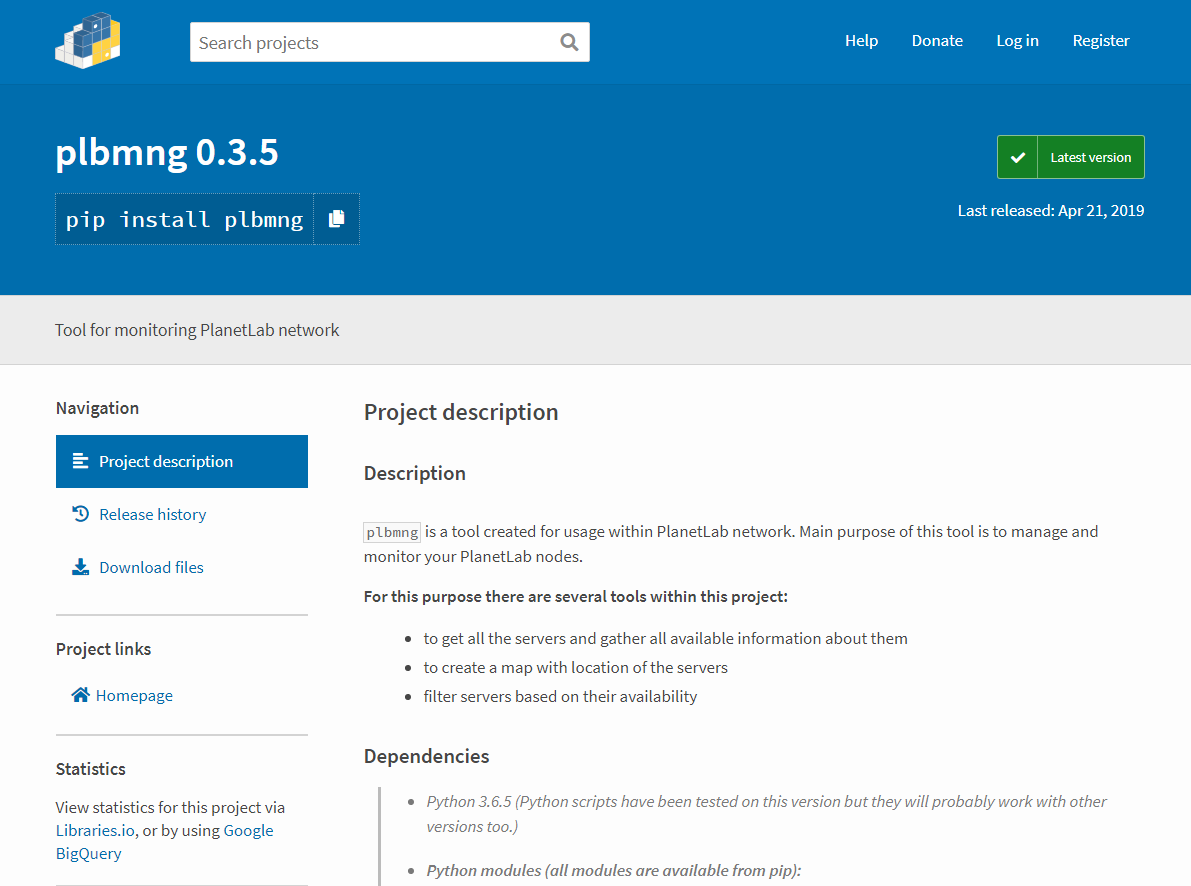
\includegraphics{obrazky/plbmng_repo}}
	\caption{New PlanetLab Server Manager web page in PyPI repository.}
	\label{fig:plbmngrepo}
\end{figure}

The installation steps are described in detail in the tool's repository page and consist of:

\begin{enumerate}
	\item Installing the application using \texttt{pip3 install plbmng} command.
	\item Starting the application using \texttt{plbmng} command.
	\item In first start it is required to set up credentials using the \texttt{Set credentials} option in menu.
\end{enumerate}

After this basic setup all the application functionality is available. It is recommended though, to update the list of nodes using \texttt{Get nodes} option in \texttt{Monitoring} menu. Installation steps are successfully reduced compared to the previous version which consisted of:

\begin{enumerate}
	\item Installing system packages using \texttt{sudo dnf install -y dialog pssh fping} command.
	\item Installing the application using \texttt{pip install plbmng} command.
	\item Locating the application in a~hidden folder of pip tool.
	\item Finding a~configuration file and using an editor to update it.
	\item Running the application using absolute path.
\end{enumerate}

\paragraph{} To summarize, current application functionality workflow diagram can be seen in Figure~\ref{fig:workflowdiagram}. For sake of diagram readability, the Figure~\ref{fig:workflowdiagram} is missing returning arrows however each node in the diagram is able to return to its parent. As seen in the Figure, first step is when menu is being initialized. From there user has option to either open \texttt{Access server menu}, \texttt{Monitor servers}, \texttt{Plot servers on map}, \texttt{Set credentials}, \texttt{About} or select \texttt{Statistics}. \texttt{Statistics} will display current data~about nodes accessibility. \texttt{About} is a~single window option that will show information about the software, its authors and license. \texttt{Set credentials} option will open an interactive editor where user can fill the credentials for PlanetLab network. Next option is \texttt{Plot servers on map} which offers user to choose which map elements should be displayed. After confirmation the map is generated and opened in the system default browser. \texttt{Monitor servers} option divides into three different options. First enables user to setup \texttt{crontab} to periodically scan for new nodes, second option is for updating status database and third updates list of nodes. At last, \texttt{Access servers} allows users to access the nodes by searching for them either using DNS name, IP address or location. After the search key is inserted, the available results are shown. It also offers user to get to last accessed node or select filtering option which are displayed on the top of the window. When specific node is chosen, information about the node are displayed and user has options to connect to the node using ssh, Midnight Commander or show the node on map. If credentials are not filled, warning message next to option is displayed.

\begin{figure}[H]
	\centering
	\scalebox{0.8}{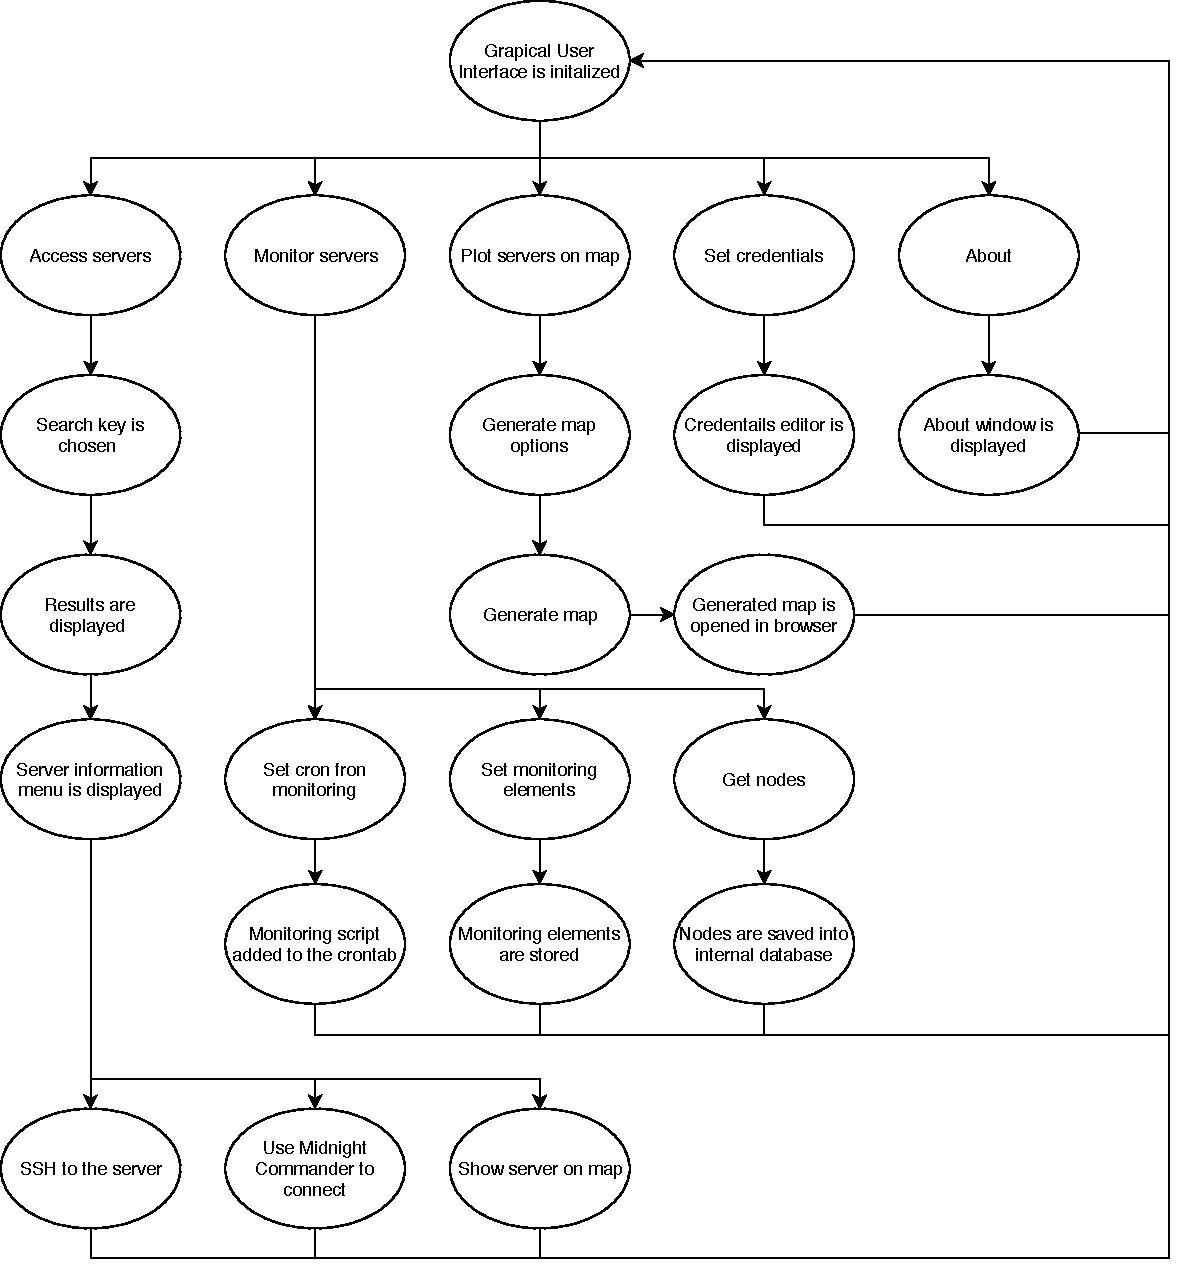
\includegraphics{obrazky/BehavioralPlbmng}}
	\caption{Behavioral diagram of new PlanetLab Server Manager.}
	\label{fig:workflowdiagram}
\end{figure}

\chapter{PlanetLab Server Manager Use Cases}
\label{chapter:usecase}
In this Chapter, various use cases of the PlanetLab Server Manager tool will be revised and described. First, analysis of the PlanetLab Network will be done in Section~\ref{section:analysis}. In Section~\ref{section:testing}, the very basic use case of the application, testing network projects in the PlanetLab Network, will be described and shown.

\section{PlanetLab Network Analysis Using Plbmng Tool}
\label{section:analysis}
In this Section, the Planet Lab network will be analyzed and discussed using the newly developed features plus using the \texttt{plbmng} database of servers pulled from the PlanetLab API. Also, data~from Chapter~\ref{chapter:planetlabnetwork} introduction will be compared to new ones with time difference of five months.\\
PlanetLab Network is a~huge project which consists of 1353 nodes at 717 sites \cite{planetlabmain}. Currently, there are around one thousand servers available to the \textit{cesnet\_utko} user from 52 countries world wide. The Figure~\ref{fig:allcountriesgraph} shows 20 countries, represented by their country code, with the most node contribution to the network which X axis showing the country and on the Y axis showing the node count for the specific country. Most of the countries are from United States with the impressive node count of 388, second is China~with its 58 nodes and third is Germany with their 49 nodes. 

\begin{figure}[H]
	\centering
	\scalebox{0.44}{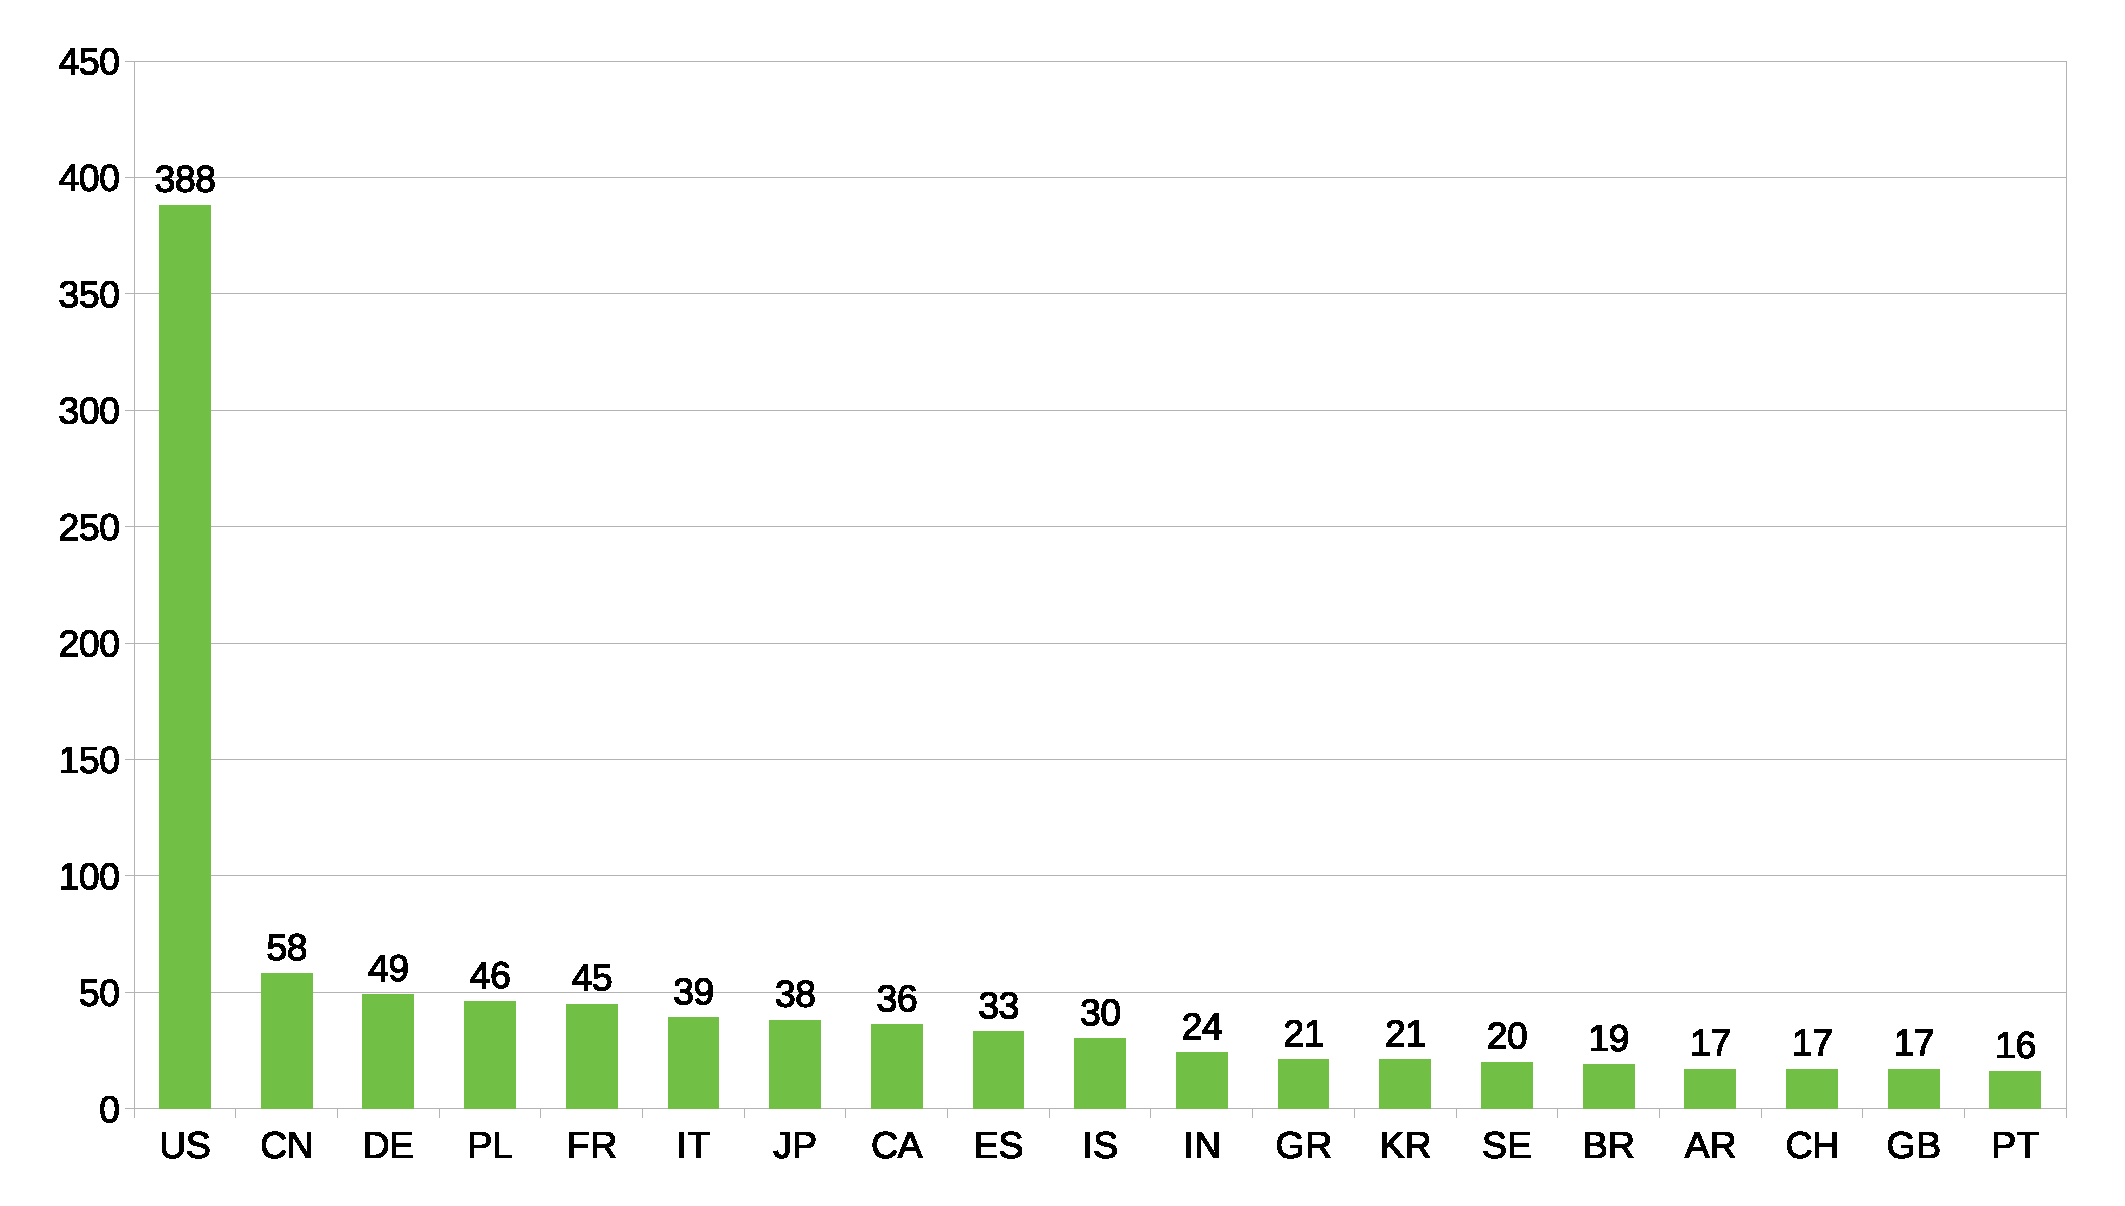
\includegraphics{obrazky/allcountriesgraph}}
	\caption{Graph displaying top twenty countries and number of nodes they have contributed to the PlanetLab Network.}
	\label{fig:allcountriesgraph}
\end{figure}

Geographically, the nodes are all over the world and are more then suitable to test large scale network project requiring multiple servers in different locations all over the world. All the nodes on a~world map can be seen in Figure~\ref{fig:allnodes} which was created using \texttt{plbmng} application.

\begin{figure}[H]
	\centering
	\scalebox{0.55}{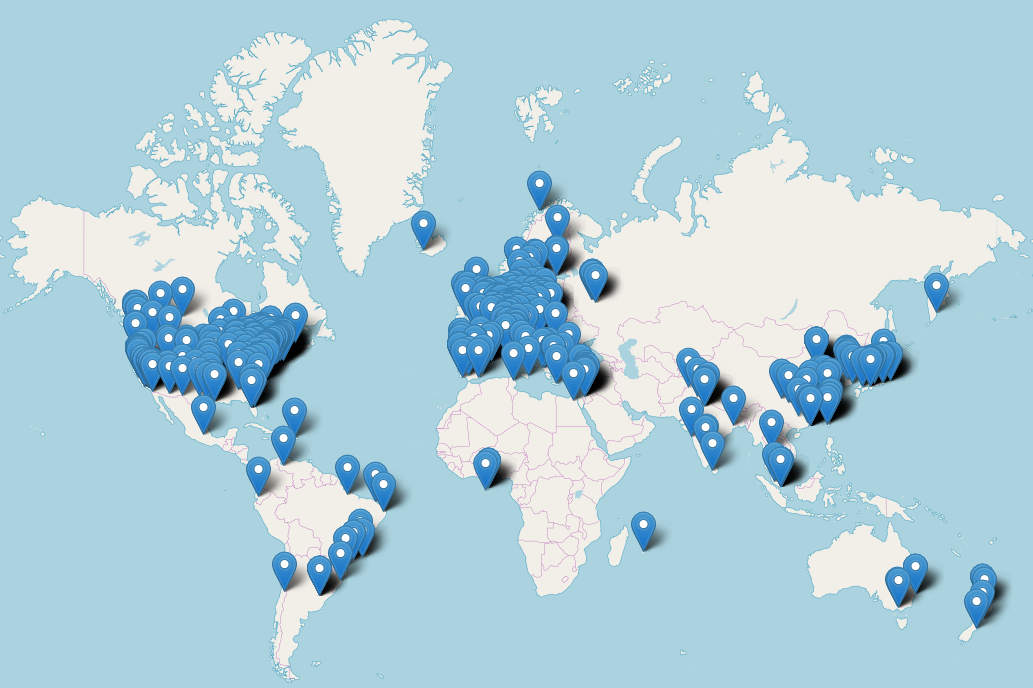
\includegraphics{obrazky/plbmng_all_nodes}}
	\caption{Nodes displayed on world map using the PlanetLab Server Manager map rendering functionality \cite{OpenStreetMap}. Data~from April 2019.}
	\label{fig:allnodes}
\end{figure}

However, not all the nodes are available. As seen in Figure~\ref{fig:nodestats}, from the database 1004 nodes only 168 nodes are responding to ICMP packets and only 140 are listening on port 22 which is usually used for ssh. That is a~very low availability percentage of only \SI{16.7}{\percent} nodes responding to ping and even less \SI{13.9}{\percent} listening on port 22. Interesting is also that 28 nodes stopped responding to ICMP packets since last measurement done in November 2018 as seen in Figure~\ref{fig:pingablepie}. That is extremely low number of available nodes and shows that the universities that are offering their nodes often do not maintain them to make sure these are still available or have left the project without decommissioning the node in the PlanetLab interface. Also, an interesting fact is that there are 28 nodes that are responding to ICMP packets but are not listening on port 22. Explanation can lie in stuck \texttt{sshd} agent or some network restrictions which are preventing to access the port 22 on specific server.

\begin{figure}[H]
	\centering
	\scalebox{0.95}{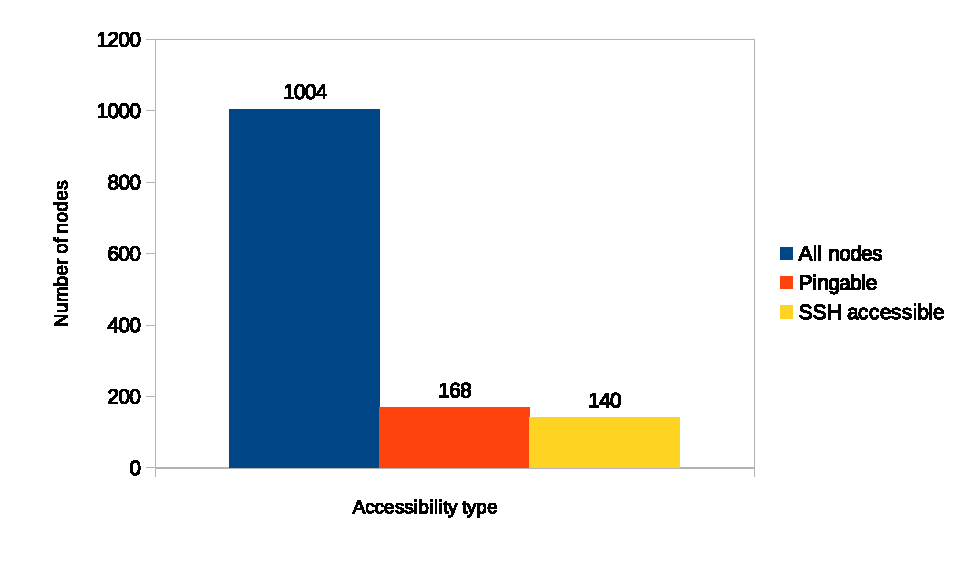
\includegraphics{obrazky/nodestats}}
	\caption{Number of PlanetLab nodes logically divided by their accessibility. Data~from April 2019.}
	\label{fig:nodestats}
\end{figure}

If data~are divided by continents, we will get graph with \texttt{ssh} accessible nodes in Figure~\ref{fig:sshcountriesgraph}. On the X axis, you can see continents and on the Y axis you can see number of accessible nodes on that particular continent. For Europe and America, the numbers are very similar. Interesting is that from South America, only 6 nodes are accessible and all are from Brazil.

\begin{figure}[H]
	\centering
	\scalebox{0.95}{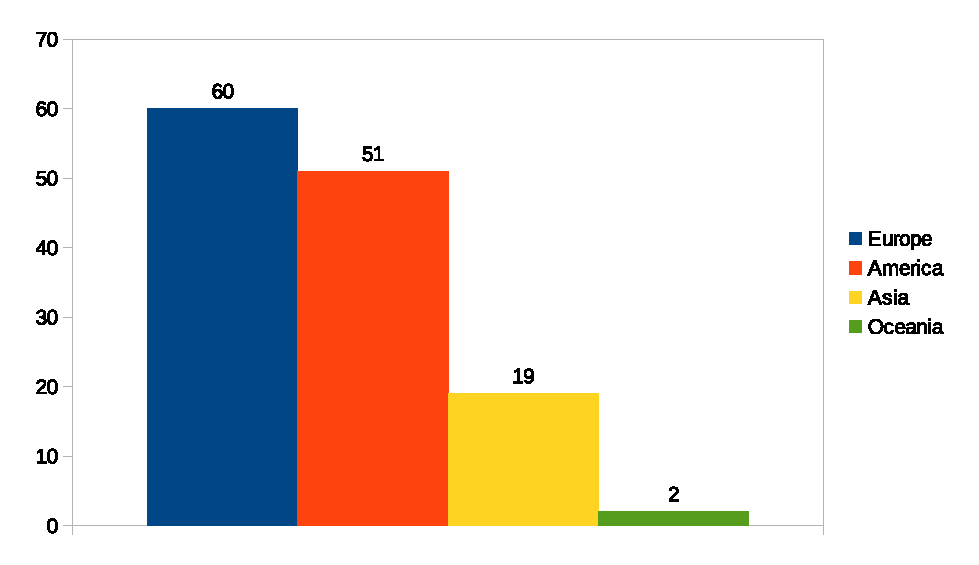
\includegraphics{obrazky/sshcountriesgraph}}
	\caption{Number of ssh accessible nodes logically divided into continents.}
	\label{fig:sshcountriesgraph}
\end{figure}

In more detailed breakdown, that can be seen in  Table~\ref{table:continentavailability}, it can be observed that Europe, with its \SI{12}{\percent}, has the biggest percentage of ssh-accessible servers compared to overall number of nodes of all continents. Ssh accessible node means node available for project testing. On the other hand, the lowest percentage of available server has China~with only \SI{10.7}{\percent}.

\begin{table}[htb]
		\resizebox{\textwidth}{!}{
				\begin{tabular}{|c|c|c|c|c|c|c|c|}
					\hline
					\rowcolor[HTML]{C0C0C0} 
					\multicolumn{2}{|c|}{\cellcolor[HTML]{C0C0C0}Europe} & \multicolumn{2}{c|}{\cellcolor[HTML]{C0C0C0}America} & \multicolumn{2}{c|}{\cellcolor[HTML]{C0C0C0}Asia} & \multicolumn{2}{c|}{\cellcolor[HTML]{C0C0C0}Oceania} \\ \hline
					\rowcolor[HTML]{EFEFEF} 
					All nodes              & Ssh accessible              & All nodes              & Ssh accessible              & All nodes             & Ssh accessible            & All nodes              & Ssh accessible              \\ \hline
					332                    & 60                          & 422                    & 51                          & 177                   & 19                        & 18                     & 2                           \\ \hline
					\SI{100}{\percent}                  & \SI{18.6}{\percent}                      & \SI{100}{\percent}                  & \SI{12}{\percent}                        & \SI{100}{\percent}                 & \SI{10.7}{\percent}                    & \SI{100}{\percent}                  & \SI{11.1}{\percent}                      \\ \hline
				\end{tabular}
		}
\centering
\caption{Table comparing number of all nodes versus ssh accessible nodes per continent using plbmng status database.}
\label{table:continentavailability}
\end{table}

When map with all nodes, seen in Figure~\ref{fig:allnodes}, is compared to map with only ssh accessible nodes, seen in Figure~\ref{fig:sshnodes}, the difference is even more clear. Map rendering functionality can be used to plan project testing and offers filtering only ssh available nodes.

\begin{figure}[H]
	\centering
	\scalebox{0.55}{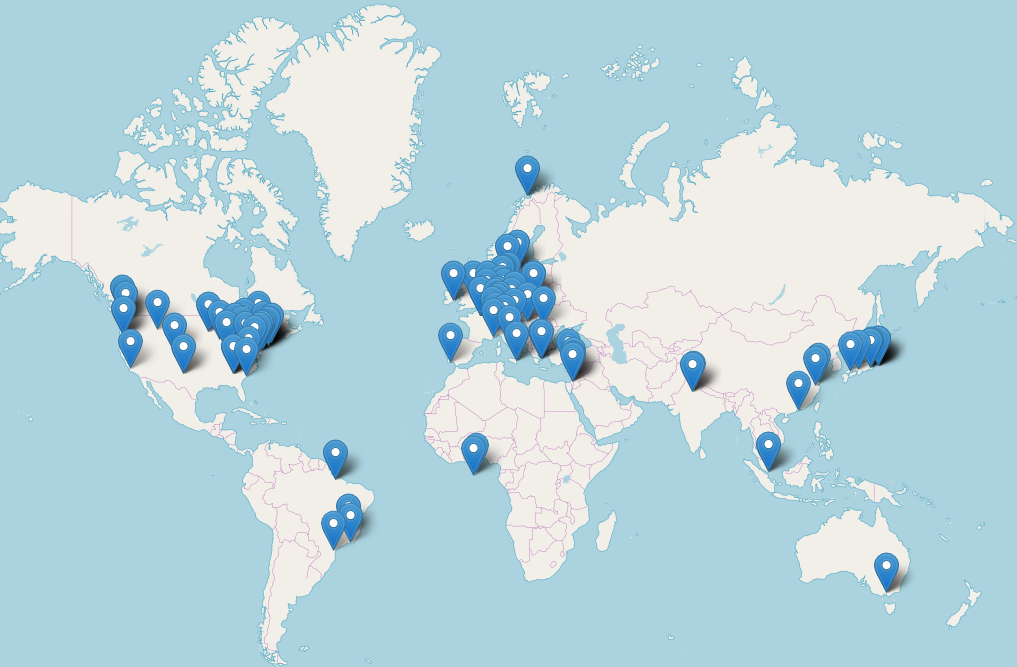
\includegraphics{obrazky/plbmng_ssh_nodes}}
	\caption{World map displaying only ssh-accessible nodes using application database \cite{OpenStreetMap}. Data~from April 2019.}
	\label{fig:sshnodes}
\end{figure}


\section{Testing Network Projects with Planet Lab Server Manager}
\label{section:testing}
In this Section, a~use case of testing a~network projects, on of the most crucial use cases, will be shown and illustrated. For the purpose of illustration a~simple imaginary project of running a~listener on port 8765 in America~and accessing it from China~and Europe will be described. The idea~of the project is to record the times that are required to establish a~connection and log necessary turn-around time for a~packet to travel between continents. Mentioned project is basically a~simple implementation of \texttt{ping} tool.\\
As a~first step, credentials needs to be updated in the \texttt{Set credentials} menu options. Next, filter is turned on to show only ssh accessible servers in the \texttt{Access servers} menu section. Later, a~server is found using the \texttt{Search by location} menu option and credentials are verified. If the connection is successful, testing can continue. For this purposes, simple Python script will be used. There will be a~server as seen in Listings~\ref{lst:echoserver} and client as seen in Listings~\ref{lst:echoclient} which all are inspired from \texttt{cyberciti.biz} site \cite{ports}. Server will be listening on port 8765 address 0.0.0.0 and client will send a~packet with message "\texttt{Test successful.}" that will be send back to the client from the server as an echo reply. The results can be seen in Figure~\ref{fig:testingusecase} where, in the terminal, three consecutive runs of plbmng application were started and using the filter and \texttt{Search by location} menu option the ssh available servers from America, China~and Europe were found and connected into. On the bottom, server from America~is shown running the echo server script. On the top left, server from China~is shown running the echo client script and on the right top corner the server from Europe is shown running also echo client script. 

\begin{figure}[H]
	\centering
	\scalebox{0.42}{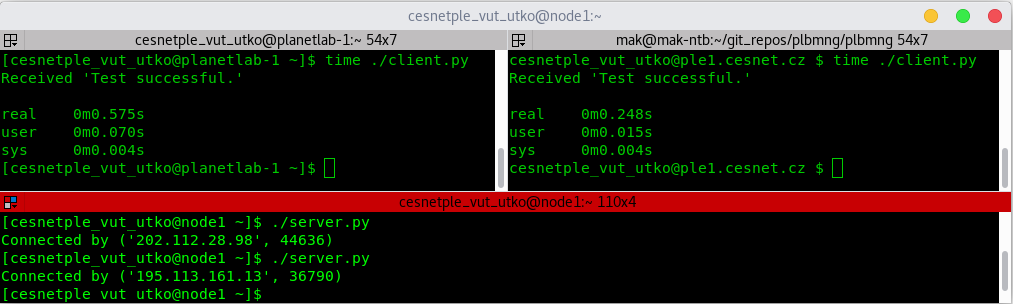
\includegraphics{obrazky/testingusecase}}
	\caption{Terminal view illustrating usage of PlanetLab Server Manager to find proper servers and run server/client echo script on them to measure round times of packets between Europe, China~and America.}
	\label{fig:testingusecase}
\end{figure}

Script was copied into servers using Midnight Commander which provides extensive interface for managing files on both local and remote locations and can be seen in Figure~\ref{fig:midnightcommander}. As you can see by the results, the packets were successfully delivered and the packet round time were 0.248 seconds for Europe and 0.575 second for the China. This use case demonstrate very simple project but the same use case can be applied basically to any project as long as it use existing tools available on the servers. Even though only a~bit above \SI{10}{\percent} servers are available, PlanetLab still offers a~vast network of nodes for project testing.

\begin{figure}[H]
	\centering
	\scalebox{0.55}{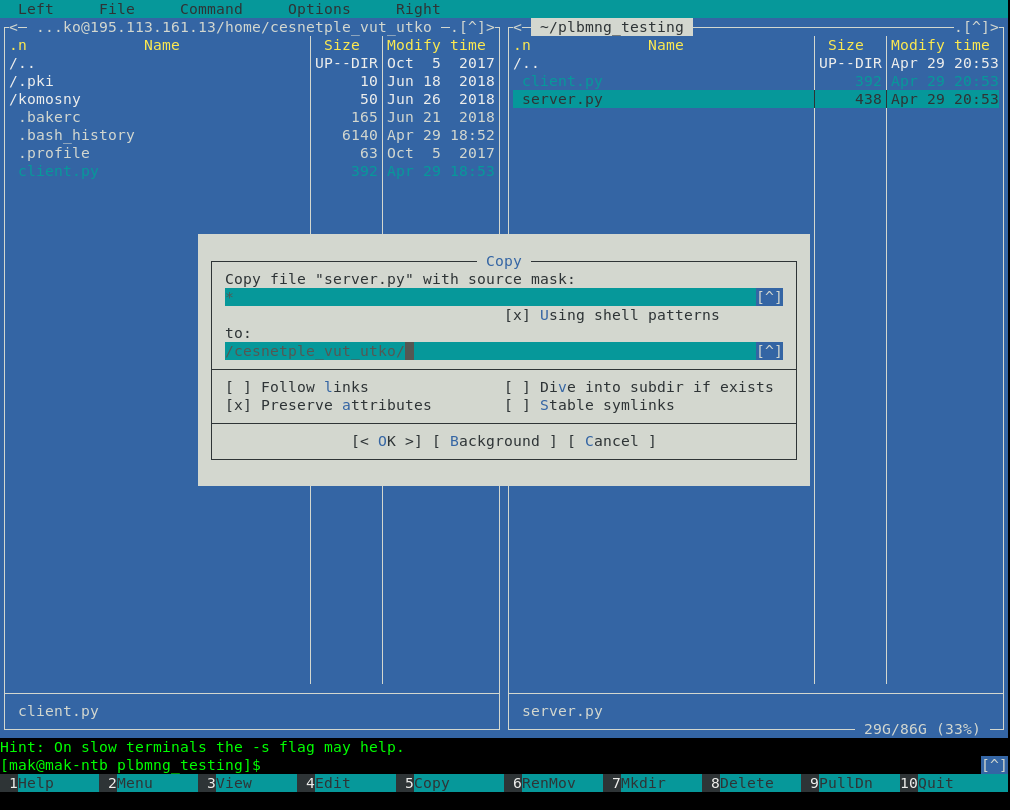
\includegraphics{obrazky/midnightcommander}}
	\caption{Illustration of midnight commander used to copy scripts from localhost (green rectangle) to a~remote server (red rectangle) inside the PlanetLab network.}
	\label{fig:midnightcommander}
\end{figure}

{\noindent\begin{minipage}{\linewidth}
		\begin{lstlisting}[language=Python, numbers=left, label={lst:echoserver}, caption=Code of echo server., frame=single, showstringspaces=false, keywordstyle=\color{blue},captionpos=b]
#!/usr/bin/python

#Demo echo server for use case example
import socket

SOURCE_HOST = source_server_ip
PORT = 8765

s~= socket.socket(socket.AF_INET, socket.SOCK_STREAM)
s.bind((SOURCE_HOST, PORT))
s.listen(1)
conn, addr = s.accept()
print 'Connected by: ', addr
while 1:
	data~= conn.recv(1024)
	if not data:
		break
	conn.send(data)
	conn.close()
		\end{lstlisting}
	\end{minipage}

{\noindent\begin{minipage}{\linewidth}
		\begin{lstlisting}[language=Python, numbers=left, label={lst:echoclient}, caption=Code of echo client., frame=single, showstringspaces=false, keywordstyle=\color{blue},captionpos=b]
#!/usr/bin/python

#Demo echo client for use case example
import socket

TARGET_HOST = target_server_ip
PORT = 8765

s~= socket.socket(socket.AF_INET, socket.SOCK_STREAM)
s.connect((TARGET_HOST, PORT))
s.send('Test successful.')
data~= s.recv(1024)
s.close()
print 'Received: ', repr(data)
		\end{lstlisting}
\end{minipage}

%% Vložení souboru 'text/zaver' se závěrem
\chapter{Conclusion}
Goal of this Master thesis was to improve the current of state of the PlanetLab Server Manager (plbmng). PlanetLab Server Manager supports research and development of distributed network services. Application was described in Chapter~\ref{chapter:planetlabnetwork}. The previous PlanetLab Server Manager tool is, in Chapter~\ref{chapter:plbmng}, reviewed, analyzed and weak points like program disparity, numerous bugs, result limitation, pre and post installation steps and others were identified and possible improvements were suggested. Since the PlanetLab network is primarily using Linux and virtualization, these technologies were covered in Subsection~\ref{subsection:Linux} and Subsection~\ref{subsection:Virtualization} respectively.\\
The improvements, as the result of this thesis, are described in Chapter~\ref{chapter:improve}. First, application logic was re-defined to use Python 3 advantages and new architecture diagram can be seen in Section~\ref{section:redesign}. One of the main improvements is fast \texttt{SQLite3} database where all data are stored and independent library modules providing functionality to the core engine. Python usage has enabled various advancements, such as removing result limitation, removing pre and po installation steps, having application available as library, increased readability by having core functions logically divided in one file instead of being composed from different files into script saved and run from disk, set credentials function has been improved, functions were written in a multi-platform way, few minor bugs were fixed and minor improvements were added. Folder structure was completely re-designed to be more transparent and easily oriented. Filter function was added to help find only available nodes. Logic to update availability database in multi-processing way was implemented. Minor but useful features features like accessing last server or having statistics available in the application are improving PlanetLab Server Manager usability. Full behavioral diagram with the new improvements is available in Section~\ref{section:currentapp}.\\
Last goal was to update the application's PyPI repository\footnote{The PlanetLab Server Manager tool is available at: https://pypi.org/project/plbmng/} with new code and updated description to fit the latest information. The repository was successfully updated with the newest code increment version \texttt{0.1.10} to version \texttt{0.3.7}. The description has been updated containing latest information regarding installation process of the tool. Dependencies were removed to reflect this change. Overall, described changes will help further development of the tool and increasing its usability for the PlanetLab users helping develop new distributed network services. 

%% Vložení souboru 'text/literatura' se seznamem literatury
%% Pro sazbu seznamu literatury použijte jednu z následujících možností

%%%%%%%%%%%%%%%%%%%%%%%%%%%%%%%%%%%%%%%%%%%%%%%%%%%%%%%%%%%%%%%%%%%%%%%%%
%1) Seznam citací definovaný přímo pomocí prostředí literatura / thebibliography

\begin{literatura}{99}

\bibitem{Mistrik1951}
MISTRÍK, Jozef. \textit{Stenografia: systém Herout-Mikulík : učebnica pre odborné školy, kurzy a samoukov}. 2. úplne prepracovane vydání. Bratislava: Štátne nakladateľstvo, 1951.	
	
\bibitem{sr02/2009}
		VUT v~Brně:
    \emph{Úprava, odevzdávání a zveřejňování vysokoškolských kva\-li\-fi\-kač\-ních prací na VUT v~Brně}\/ [online].
		Směrnice rektora č.\,2/2009.
		Brno: 2009, po\-sled\-ní aktualizace 24.\,3.\,2009 [cit.\,23.\,10.\,2015].
    Dostupné z~URL:\\
    <\url{https://www.vutbr.cz/uredni-deska/vnitrni-predpisy-a-dokumenty/smernice-rektora-f34920/}>.

\bibitem{CSN_ISO_690-2011}
    \emph{ČSN ISO 690 (01 0197) Informace a dokumentace -- Pravidla pro bibliografické odkazy a citace informačních zdrojů.}
    40 stran. Praha: Český normalizační institut, 2011.

\bibitem{CSN_ISO_7144-1997}
    \emph{ČSN ISO 7144 (010161) Dokumentace -- Formální úprava disertací a podobných dokumentů.}
    24 stran. Praha: Český normalizační institut, 1997.

\bibitem{CSN_ISO_31-11}
    \emph{ČSN ISO 31-11 Veličiny a jednotky -- část 11: Matematické znaky a značky používané ve fyzikálních vědách a v~technice.}
    Praha: Český normalizační institut, 1999.

\bibitem{BiernatovaSkupa2011:CSNISO690komentar}
    BIERNÁTOVÁ, O., SKŮPA, J.:
    \emph{Bibliografické odkazy a citace dokumentů dle ČSN ISO 690 (01 0197) platné od 1.\,dubna 2011}\/ [online].
    2011, poslední aktualizace 2.\,9.\,2011 [cit. 19.\,10.\,2011].
    Dostupné z~URL:
    \(<\)\url{http://www.citace.com/CSN-ISO-690.pdf}\(>\)
%    \(<\)\href{http://www.boldis.cz/citace/citace.html}{http://www.boldis.cz/citace/citace.html}\(>\).

\bibitem{pravidla}
    \emph{Pravidla českého pravopisu}.
    Zpracoval kolektiv autorů. 1.\ vydání.
    Olomouc: FIN PUB\-LISH\-ING, 1998. 575 s. ISBN 80-86002-40-3.

\bibitem{Walter1999}
	WALTER, G.\,G.; SHEN, X.
	\emph{Wavelets and Other Orthogonal Systems}.
	2. vyd. Boca Raton: Chapman\,\&\,Hall/CRC, 2000. 392~s. ISBN 1-58488-227-1

\bibitem{Svacina1999IEEE}
	SVAČINA, J.
	Dispersion Characteristics of Multilayered Slotlines -- a Simple Approach.
	\emph{IEEE Transactions on Microwave Theory and Techniques},
	1999, vol.\,47, no.\,9, s.\,1826--1829. ISSN 0018-9480.

\bibitem{RajmicSysel2002}
    RAJMIC, P.; SYSEL, P.
    Wavelet Spectrum Thresholding Rules.
    In \emph{Proceedings of the International Conference Research in Telecommunication Technology},
    Žilina: Žilina University, 2002. s.\,60--63. ISBN 80-7100-991-1.

\end{literatura}


%%%%%%%%%%%%%%%%%%%%%%%%%%%%%%%%%%%%%%%%%%%%%%%%%%%%%%%%%%%%%%%%%%%%%%%%%
%%2) Seznam citací pomocí BibTeXu
%% Při použití je nutné v TeXnicCenter ve výstupním profilu aktivovat spouštění BibTeXu po překladu.
%% Definice stylu seznamu
%\bibliographystyle{unsrturl}
%% Pro českou sazbu lze použít styl czechiso.bst ze stránek
%% http://www.fit.vutbr.cz/~martinek/latex/czechiso.tar.gz
%%\bibliographystyle{czechiso}
%% Vložení souboru se seznamem citací
%\bibliography{text/literatura}
%
%% Následující příkaz je pouze pro ukázku sazby literatury při použití BibTeXu.
%% Způsobí citaci všech zdrojů v souboru odkazy.bib, i když nejsou citovány v textu.
%\nocite{*}
\makeatletter
\def\@openbib@code{\addcontentsline{toc}{chapter}{Bibliography}}
\makeatother
\bibliographystyle{czplain}
\begin{flushleft}
\bibliography{text/literatura_mak} % viz. literatura.bib
\end{flushleft}


%% Vložení souboru 'text/zkratky' se seznam použitých symbolů, veličin a zkratek
\begin{seznamzkratek}{KolikMista}

	\novazkratka{zkDNS}
		{DNS}
		{Domain Name System}
		
	\novazkratka{zkIP}
		{IP}
		{Internet Protocol}
		
	\novazkratka{zkKVM}
		{KVM}
		{Kernel-based Virtual Machine}
		
	\novazkratka{zkMMU}
		{MMU}
		{Memory Management Unit}
		
	\novazkratka{zkCPU}
		{CPU}
		{Central Processing Unit}
		
	\novazkratka{zkCENTOS}
		{CentOS}
		{Community Enterprise Operating System}


\end{seznamzkratek}


%% Začátek příloh
%\prilohy

%% Vysázení seznamu příloh
%\seznampriloh

%% Vložení souboru 'text/prilohy' s přílohami
%\chapter{Content of DVD}
As a part of this thesis there is a CD which contains following items:
\begin{itemize}
	\item Latex source codes in folder \texttt{latex}.
	\item Text version of the thesis in pdf format.
	\item The application in folder \texttt{plbmng}.
\end{itemize}

\chapter{Manual}
This appendix contains manual for the application implemented in this thesis. It describes how to run the application either using source codes on the attached CD or using PyPI repositories. The application was tested on \texttt{Python version 3.7.3}.
\section{Installation from PyPI repositories and running the application}
To install and run application using PyPI repositories, please do the following:\\
\begin{enumerate}
	\item In your terminal run \texttt{pip3 install plbmng}
	\item Confirm that you want to also install dependencies
	\item Once done just start application using command \texttt{plbmng}
\end{enumerate}

\section{Running application from CD}
To run application using source codes on the attached CD please do the following:\\
\begin{enumerate}
	\item In your terminal navigate into the CD folder: \texttt{cd \$CD\_FOLDER}
	\item Navigate into source code folder: \texttt{cd plbmng}
	\item Run the application: \texttt{./bin/plbmng}
\end{enumerate}

%% Konec dokumentu
\end{document}
